% ================================================
% =                 METHODOLOGY                  =
% ================================================ 
This section details the methodology and implementations undertaken to address the objectives described in Section~\ref{sec:objectives}. On the first hand, the pipeline design for addressing \textit{"wich is the best approach for segmenting planar elements"} is introduced, tackling the model and dataset selection and the training and validation processes. Afterward, the implementation of the occupancy, occlusion, and drivable area pre-annotation pipeline is presented. Finally, the evaluation strategy of the pipeline is discussed to measure the quality of the resulting semantic masks and the monocular 3D detections for estimating the object's dimensions.

Thus, this project can be divided into two main blocks: \aclink{BEV} semantic segmentation experimentation and the design and implementation of the pre-annotation pipeline. Finally, all experiments for evaluating the models and the resulting framework are presented.  

\subsection{Segmentation experiment design: BEV2Seg\_2} \label{sec:bev2seg_2}

To address the hypotesis that \textit{A semantic segmentation model trained with \aclink{BEV} images better segments planar elements} the process represented in Figure~\ref{fig:beg2seg_2_flow} has been designed. It follows two main approaches: first, performing image segmentation on regular RGB images and then reprojecting them to \aclink{BEV}; second, applying \aclink{IPM} to the original images and then segmenting them with the model.

\begin{figure}[h!]
    \centering
    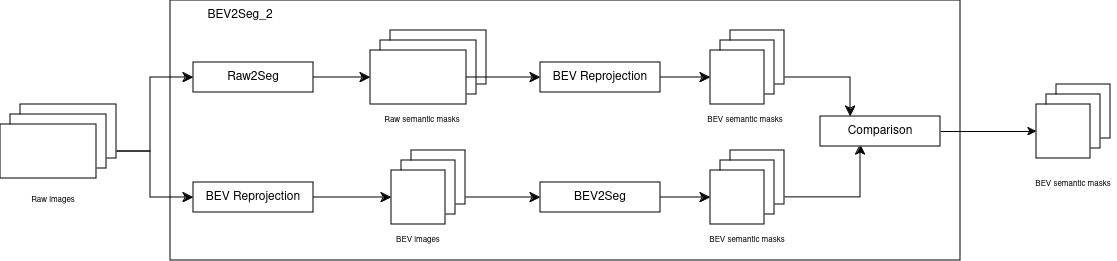
\includegraphics[width=\linewidth]{./images/methodology/bev2seg_2_flow.png}
    \caption{bev2seg\_2 flow diagram.}
    \label{fig:beg2seg_2_flow}
\end{figure}

Considering this flowchart, three main questions arises: (1) which segmentation model to use, (2) which dataset to train the models with, and (3) how to compare the train models and select the optimal output of the pipeline. 

\subsubsection{Segformer}
There are multiple techniques and strategies for tackling semantic segmentation in both regular and \aclink{BEV} images (see Section~\ref{sec:sota}).  

Several models could be chosen to address the proposed hypothesis. The current state of the art includes both \aclink{CNN} and \aclink{ViT}-based models that achieve competitive results. As shown in Figure~\ref{tab:segformer_model_comparison}, there is no significant difference in accuracy and inference speed among the top-performing models. Moreover, many of these models have already been applied in the context of \aclink{ADS}. In this work, Segformer~\cite{segformer} has been selected as the semantic segmentation model due to its balance between performance and efficiency. Additionally, it is integrated into the Huggingface~\cite{huggingface} ecosystem, which provides an optimized, parallelized implementation, facilitating distributed training.  

\begin{table}[h]
    \centering
    \resizebox{\linewidth}{!}{%
    \begin{tabular}{l l c c c}
        \toprule
        \textbf{Model Name} & \textbf{Encoder} & \textbf{Params (M)} $\downarrow$ & \textbf{FPS} $\uparrow$ & \textbf{Cityscapes test mIoU ($\%$)} $\uparrow$ \\
        \midrule
        DDRNet-39       & -             & 32.3      & -         & 80.4 \\
        PIDNet-L        & -             & 36.9      & -         & 80.6 \\      
        DeeplabV3+      & ResNet-101    & 62.7      & 1.2       & 80.9 \\
        SETR            & ViT-Large     & 318.3     & 0.5       & 82.2 \\
        Segformer       & MiT-B4        & 64.1      & 3.0       & 83.8 \\
        \bottomrule
    \end{tabular}%
    }
    \caption{Comparison of different models. Results are obtained from \cite{DDRNet} \cite{PIDNet} \cite{segformer}.  }
    \label{tab:segformer_model_comparison}
\end{table}


The Segformer model consists on an hierarchical Transformer  encoder, which extract coarse and fine features, and a lightweight \aclink{MLP} decoder to directly fuse these multiscale features and predict the segmentation mask (Figure~\ref{fig:segformer_architecture}). Segformer comes with a series of Mix Transformer encoders (MiT) that share the same architecture but have different sizes: from MiT-B0 as the lightweigtest encoder for realtime inference, to MiT-B5 for best performance.

\begin{figure}[h!]
    \centering
    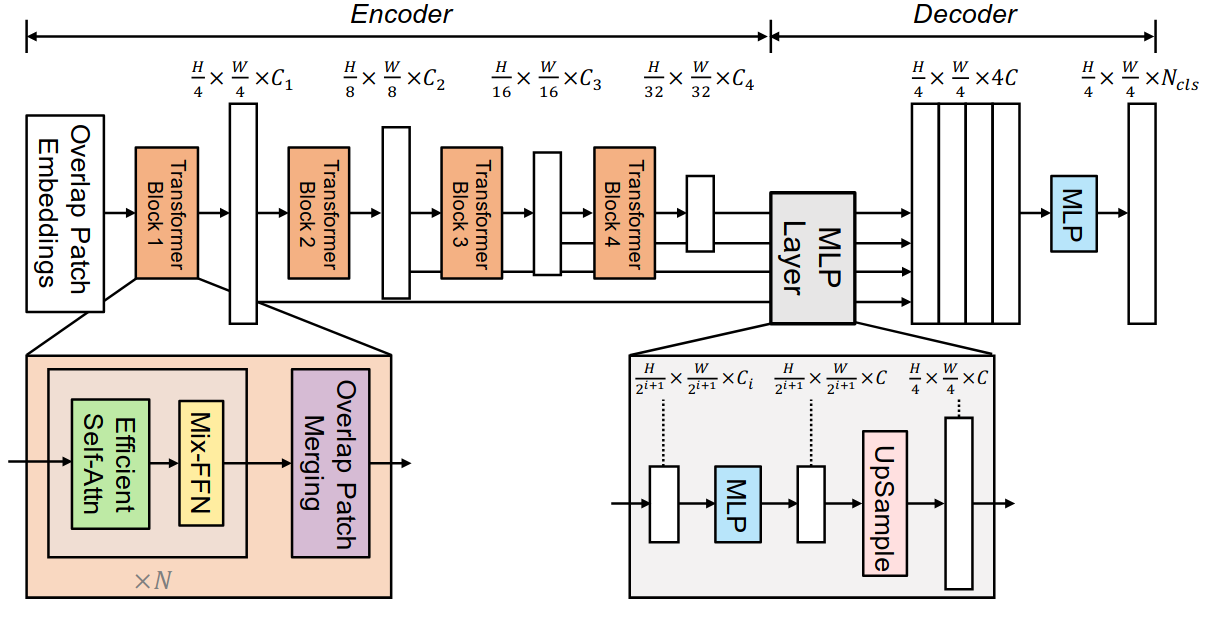
\includegraphics[width=\linewidth]{images/methodology/segformer_architecture.png}
    \caption{Segformer architecture}
    \label{fig:segformer_architecture}
\end{figure}

The training strategy involves using pretrained encoders from ImageNet-1K, attaching an untrained segmentation head decoder, and fine-tuning the entire model for semantic segmentation of vehicular scenes. Since the objective is to train the models directly on \aclink{BEV} images, which differ significantly from standard perspective images, the encoder layers will remain trainable rather than being frozen.


\subsubsection{BEVDataset} \label{sec:BEVDataset}
In order to train the model on the segmentation task, a valid dataset must be selected. There are several semantic segmentation datasets for the \aclink{ADS} context such as Cityscapes \cite{Cityscapes}, that defines $30$ semantic classes and provides $5.000$ frames with pixel-level high-quality annotations and $20.000$ weakly annotated images; KITTI \cite{KITTI}, which provices $400$ annotated images with a $0.5$ split for training and validation following the Cityscapes annotation format; ApolloScape \cite{ApolloScape}, that provides $146.997$ frames with corresponding pixel-level annonations and pose information for $25$ labels; or NuImages, a subset of NuScenes \cite{nuscenes}, that contains annotated images on $26$ different labels. For all of them, the ego pose and camera parameters metadata are provided. 

There are other benchmarks \cite{WildDash} \cite{CamVid} but in orther to train the models a rich dataset is needed. Despite Cityscapes and ApolloScape being good options for this task, NuImages has been selected as it is one of the most used datasets for \aclink{ADS} tasks, it provides very accurate ego poses and camera parameters, it has 3D annotations and it has a very good documentation.

NuImages contains around $93.000$ samples with aproximately $80\%$ reserved for the training set and $20\%$ for validation. Additionally, NuImages includes a private test set reserved for benchmark evaluations, whose annotations are not publicly available.

To train the models in the pipeline, a parser has been developed to convert NuImages into a sub-dataset named BEVDataset. This dataset has all front-camera images with NuImages annotations. Since the test annotations in NuImages are private, the validation set has been further splitted to ensure fair comparisons between models from different pipelines.

The conversion process is performed using a custom parser named 'OLDatasets', which transforms NuImages samples into the structured ASAM OpenLABEL \footnote{\url{https://www.asam.net/standards/detail/openlabel/}} format, where metadata for each frame is stored. In the case of BEVDataset, images are reprojected into the \aclink{BEV} domain using the \aclink{VCD} library \cite{VCD}. This library provides tools to handle OpenLABEL annotations and manage both 2D and 3D data efficiently.

The OLDatasets parser extracts the camera parameters for each sample and computes a lookup table to apply \aclink{IPM} reprojection. Using this data, semantic pixel masks are generated and reprojected along with the original images into the \aclink{BEV} space. Since this reprojection involves image warping, the interpolation method must be carefully chosen:
\begin{itemize}
    \item Linear interpolation is applied to images.
    \item Nearest neighbor interpolation is used for semantic masks to preserve pixel class integrity. 
\end{itemize}

The virtual \aclink{BEV} camera parameters are fixed. The reprojection's coordinate system origin is set as the midpoint of the rear wheel's axle, according to the ISO 8855 standard~\cite{ISO8855}. This setup projects a regular grid with a 1-meter cell spacing, spanning 30 meters in front of the vehicle and 1 meter behind it. The resulting images have a resolution of $1024 \times 1024$ pixels.

Finally, BEVDataset contains a total of $16.427$ images, distributed as shown in Figure~\ref{fig:bev_dataset}. More details about the dataset conversion and especifications can be fount at Appendix~\ref{appendix:OLDatasets}.

\begin{figure}[h!]
    \centering
    \includegraphics[width=\linewidth]{images/methodology/BEVDataset.png}
    \caption{BEVDataset structure and mini set samples}
    \label{fig:bev_dataset}
\end{figure}

\subsubsection{Validation and comparison}
When validating and comparing different segmentation models, it is essential to use a common dataset and apply appropriate metrics that allow for a quantitative and objective evaluation of model performance. The first requirement is met by using the test set of the dataset, which has not been previously exposed to the models being compared. Regarding evaluation metrics, as shown in Figure~\ref{fig:semantic_masks}, where a semantic mask predicted by a segmentation model is displayed alongside the corresponding annotated ground truth mask, it is intuitive to assume that an accurate prediction is one that maximizes the overlap between the predicted mask and the ground truth while also avoiding excessive overflow beyond the boundaries of the ground truth regions.

\begin{figure}[htbp]
    \centering
    \begin{subfigure}[b]{0.3\textwidth}
        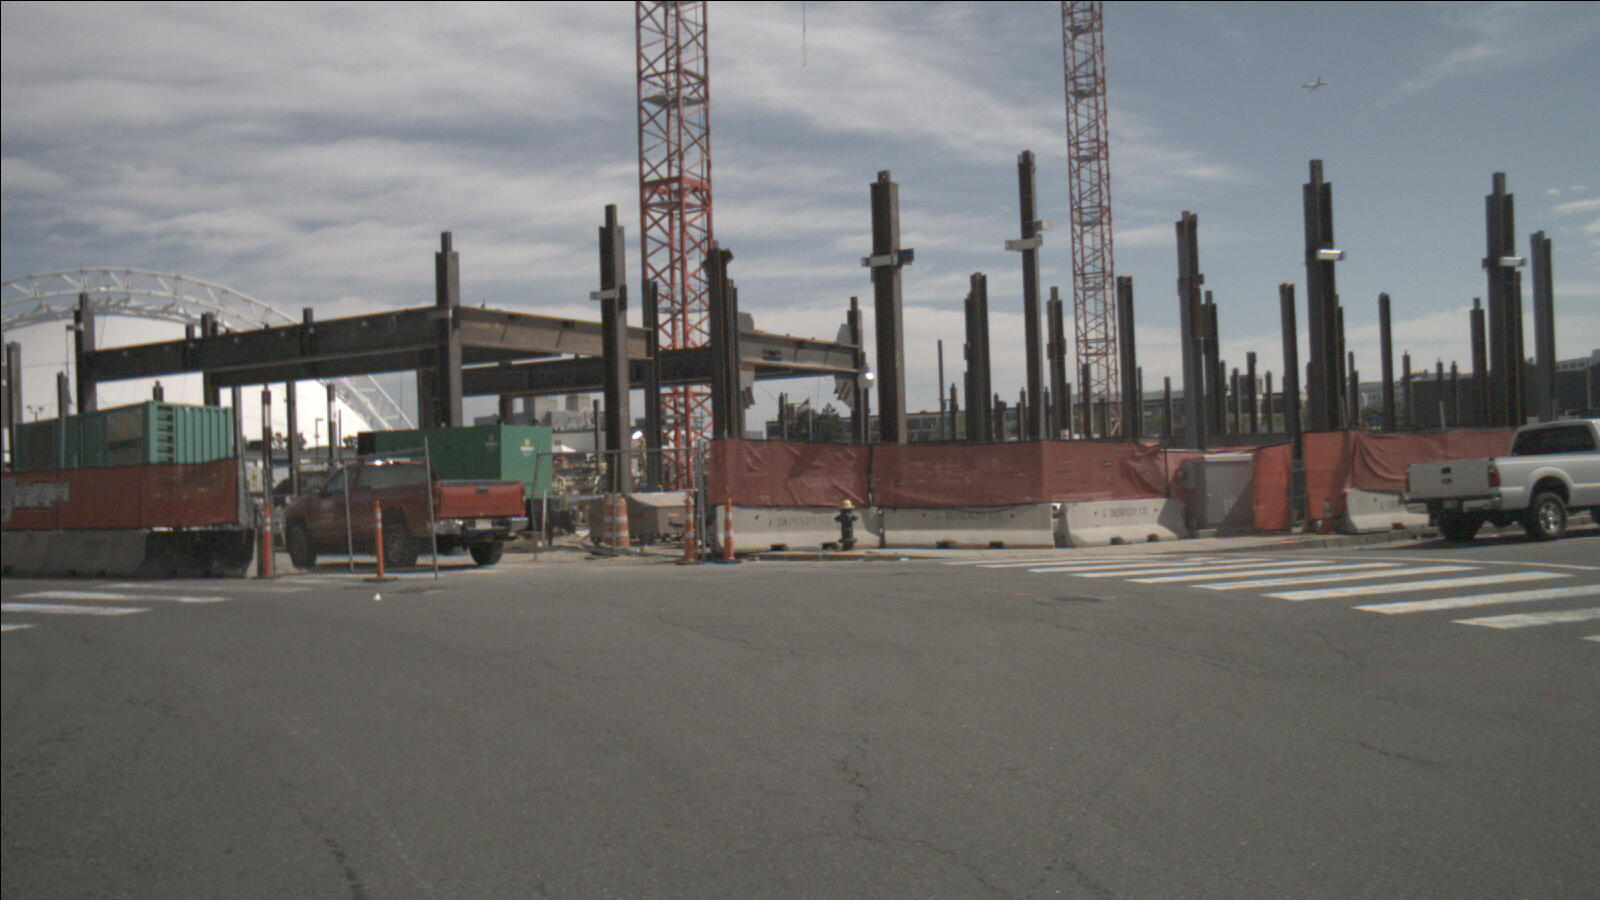
\includegraphics[width=\textwidth]{images/methodology/raw/original_image_2.png} 
        \caption{}
        \label{fig:semantic_masks_a}
    \end{subfigure}
    \hfill
    \begin{subfigure}[b]{0.3\textwidth}
        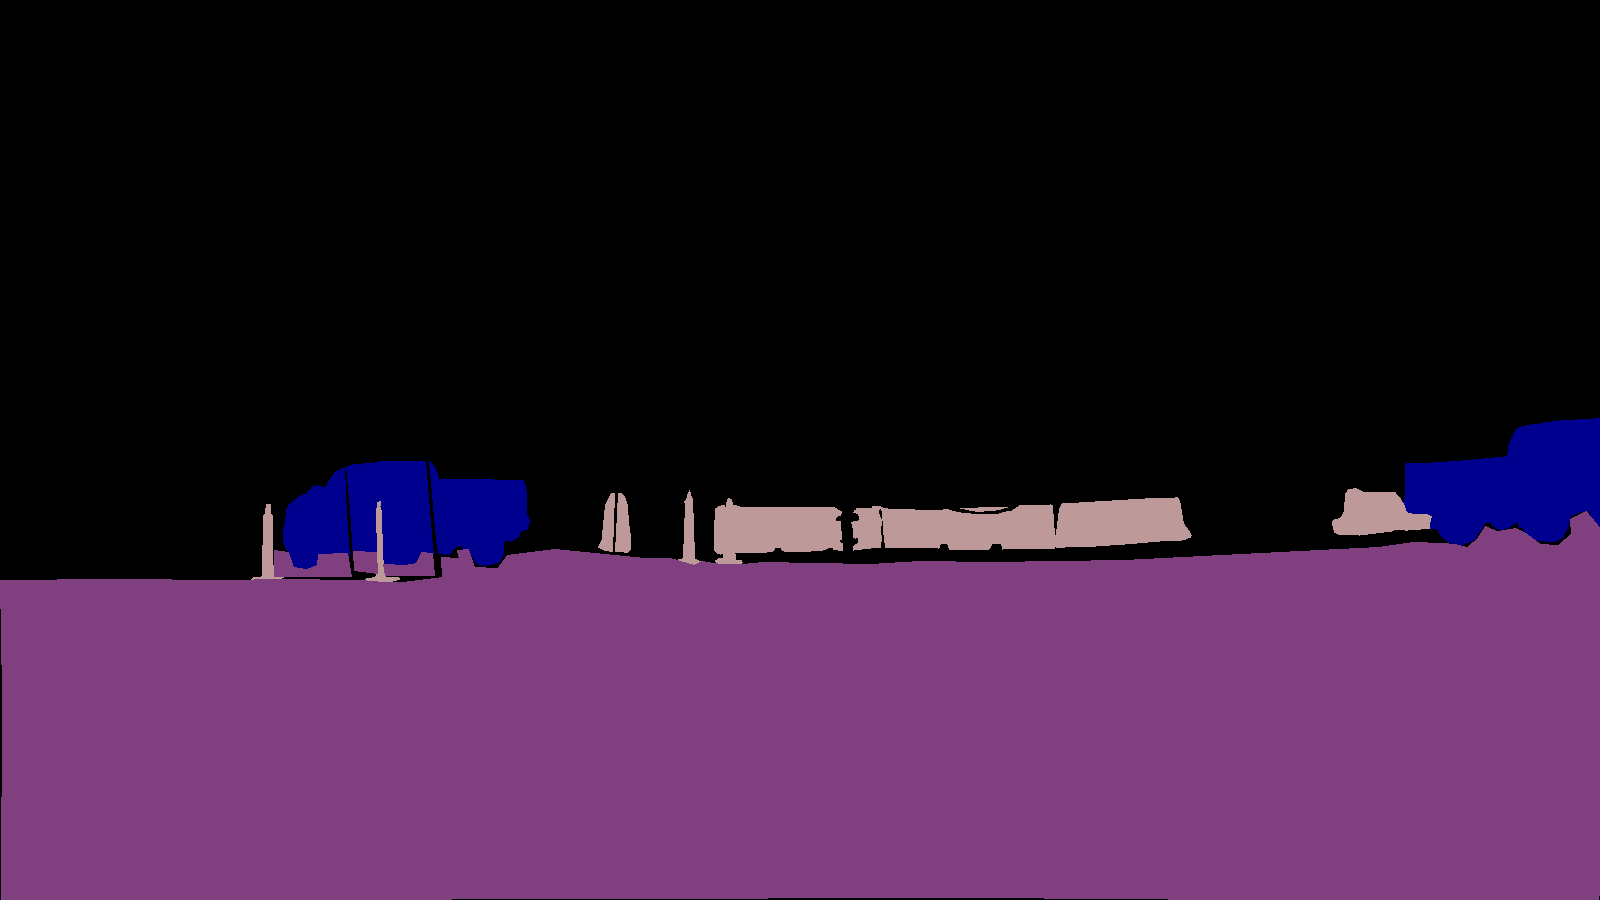
\includegraphics[width=\textwidth]{images/methodology/semantic_colored/2_target_color.png}
        \caption{}
        \label{fig:semantic_masks_b}
    \end{subfigure}
    \hfill
    \begin{subfigure}[b]{0.3\textwidth}
        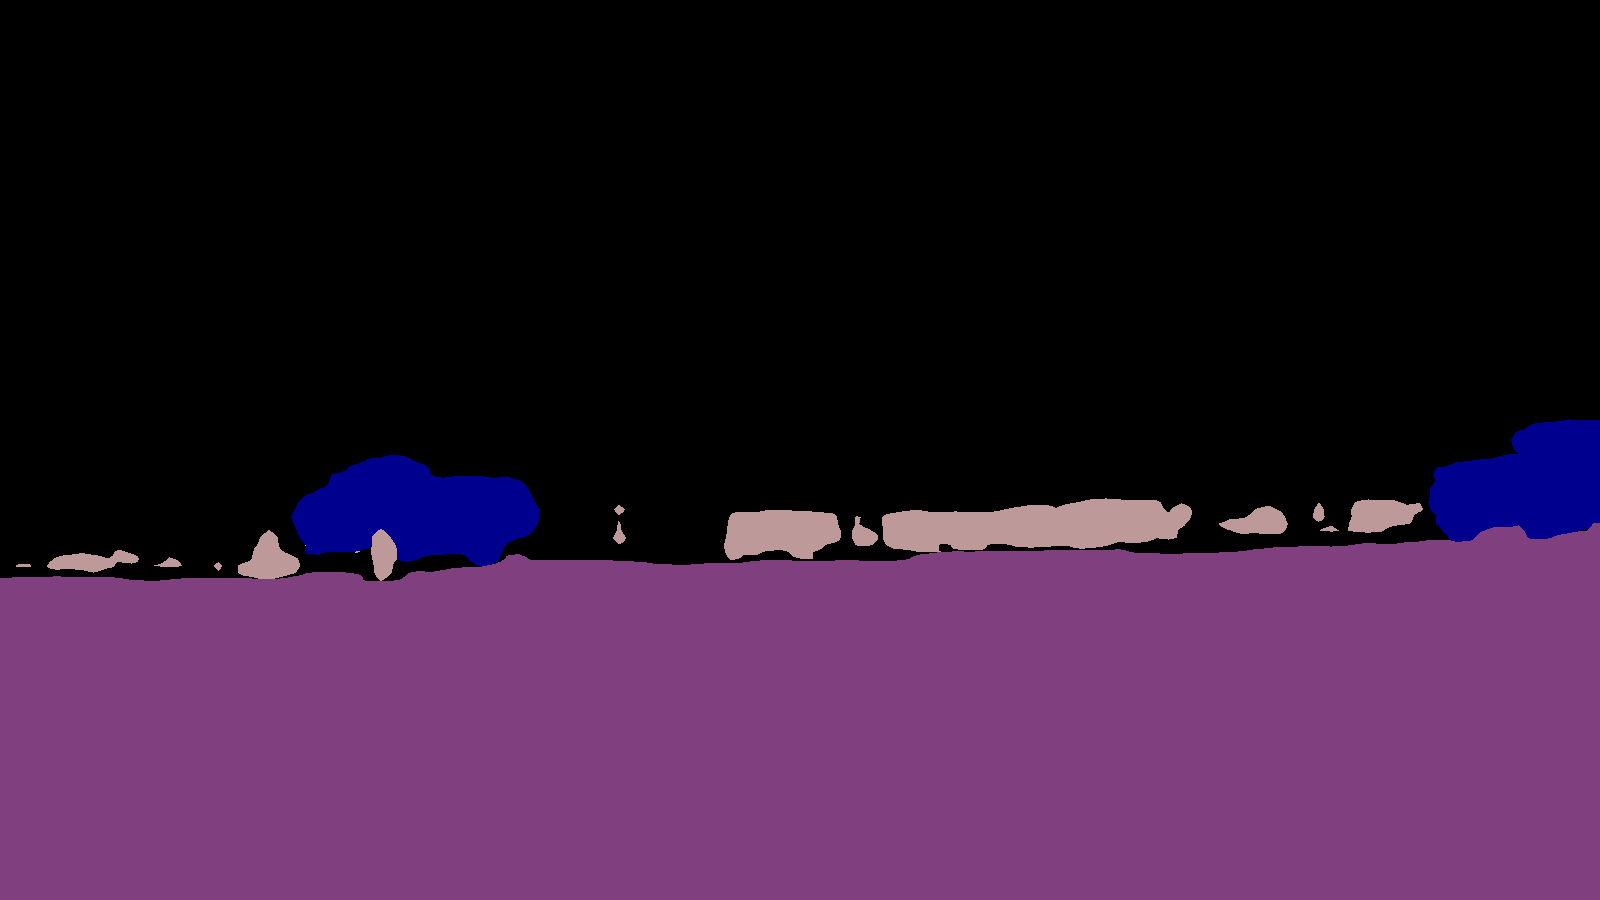
\includegraphics[width=\textwidth]{images/methodology/semantic_colored/2_inference_color.png}
        \caption{}
        \label{fig:semantic_masks_c}
    \end{subfigure}

    \caption{Semantic masks example: (a) original image, (b) colored semantic ground truth, (c) colored inferenced semantic mask.}
    \label{fig:semantic_masks}
\end{figure}

To quantify this, two distinct but related metrics are commonly used: the Dice coefficient (also known as the F1-score) and the Jaccard index, also known as \aclink{IoU}, whose formal definitions are presented in Formula~\ref{eq:semantic_metrics}. Both metrics are bounded within the range [0, 1], where 0 indicates no overlap between prediction and ground truth, and 1 indicates a perfect match between the two masks.

\begin{equation}
    \begin{aligned}
    \text{Dice}(A, B) &= \frac{2\,|A \cap B|}{|A| + |B|} = \frac{2\,TP}{2\,TP + FP + FN} \\
    \text{Jaccard}(A, B)  &= \frac{|A \cap B|}{|A \cup B|} = \frac{TP}{TP + FP + FN}
    \end{aligned}
    \label{eq:semantic_metrics}
\end{equation}

Suppose we start from an image with resolution $H \times W$ and aim to predict $N$ different classes. The model output will be a tensor of dimensions $H \times W \times N$, representing $N$ masks of size $H \times W$, where each element encodes a class-specific confidence value. However, in semantic segmentation, only the best prediction per pixel is retained, resulting in $N$ binary masks that represent the final semantic classifications of the original image. In this context, the described metrics are computed independently for each of the $N$ classes.

For a fixed ground truth, both metrics are positively correlated: if classifier A outperforms classifier B according to one metric, it will also outperform it according to the other (see Appendix~\ref{appendix:f1_iou}). This might suggest that the choice between the two metrics is arbitrary; however, differences become apparent when averaging scores over a set of predictions. At this stage, although both metrics may agree that model A performs better than model B, they differ in how much better one model is compared to the other.

In general, the \aclink{IoU} metric tends to penalize poorly classified instances more severely than the F1-score, thereby offering a performance measure that reflects worst-case behavior. In contrast, the F1-score is more representative of average-case performance. As a result, when computing averages across multiple predictions, \aclink{IoU} is more sensitive to significant outliers, while F1-score tends to be more forgiving in such cases.

Taking all this into account, \aclink{mIoU} has been chosen as the primary metric for evaluating and comparing models in this work.

\subsection{Driveable area automatic annotation}
\label{sec:aplication}

This section details the selected approach used to automatically annotate occupancy and occlusion masks in vehicular scenes. The method employs a 2D-to-3D approach, using estimated depth maps from monocular images to approximate object dimensions and compute the corresponding masks.

As shown in Figure~\ref{fig:application_flow_diagram}, the method can be divided into four main stages: depth estimation, where a depth map is generated from monocular front images; frame point cloud estimation, which creates a 3D representation of the current scene; projection of the perspective semantic mask onto the 3D point cloud to infer object instances for each selected semantic class; and the final computation of occupancy, occluded, and drivable areas by combining 3D object information with \aclink{BEV} semantic masks.

The system's output is annotated in the OpenLABEL format and integrated with the WebLABEL~\cite{weblabel} ecosystem, enabling further fine annotations by the user. Additionally, a visualization tool has been developed using the Open3D~\cite{open3d} library to facilitate the rendering process of vehicular scenes.

\begin{figure}[h!]
    \centering
    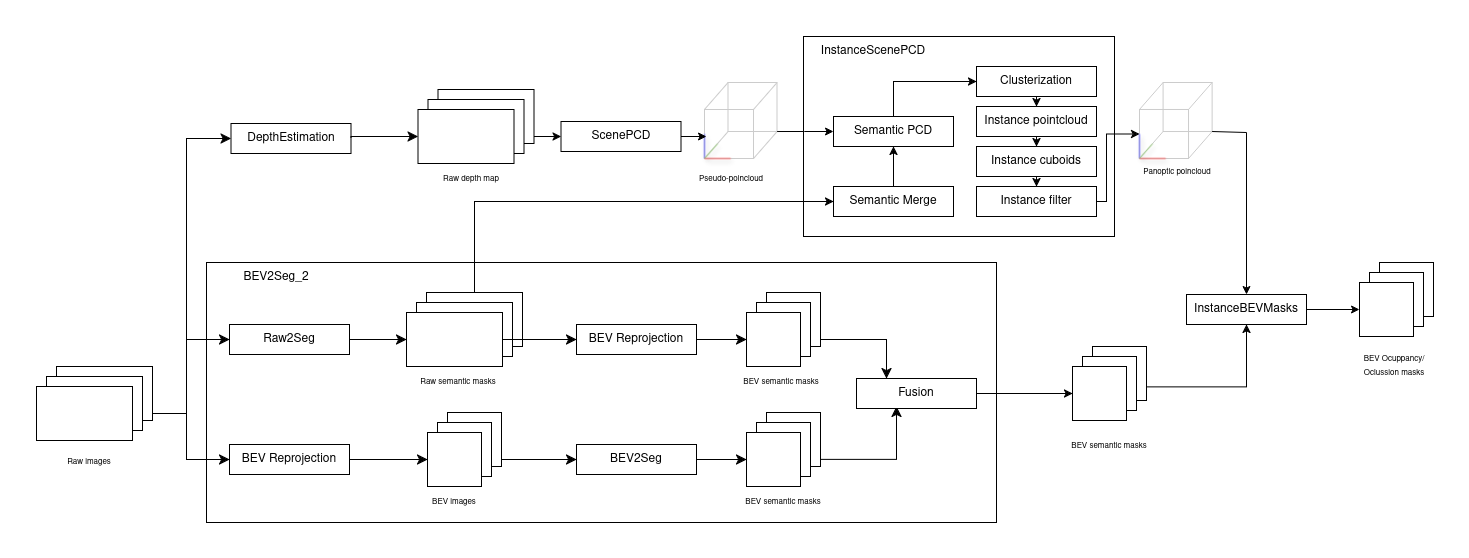
\includegraphics[width=\linewidth]{images/methodology/Application_flow_diagram.png}
    \caption{Annotation flow diagram.}
    \label{fig:application_flow_diagram}
\end{figure}

\subsubsection{Depth estimation}
\label{sec:depth_estimation}

Traditional depth estimation techniques \cite{computer_vision_depth_estimation} rely on geometric and photometric marks to infer depth from images. For example, stereo vision (\ref{fig:depth_estimation_a}) uses two or more cameras to capture the same scene from slightly different viewpoints, allowing depth to be estimated through disparity between the images. Similarly, structure from motion (SfM) (\ref{fig:depth_estimation_b}) relies on multiple images taken at different times or positions to compute motion parallax and infer scene's depth. Other multi-view techniques include shape from defocus (\ref{fig:depth_estimation_c}), which estimates depth based on the amount of blur in the images, and photometric stereo (\ref{fig:depth_estimation_d}), which uses multiple images captured from the same viewpoint but under different lighting directions to recover surface orientation and depth.

In the case of single-image depth estimation, traditional methods like shape from shading (\ref{fig:depth_estimation_e}) attempt to infer depth based on lighting and texture patterns. However, these methods typically rely on strong assumptions about the scene's geometry and lighting conditions, and thus only work reliably in controlled or well-defined environments.

\begin{figure}[htbp]
    \centering
    \begin{subfigure}[b]{0.18\textwidth}
        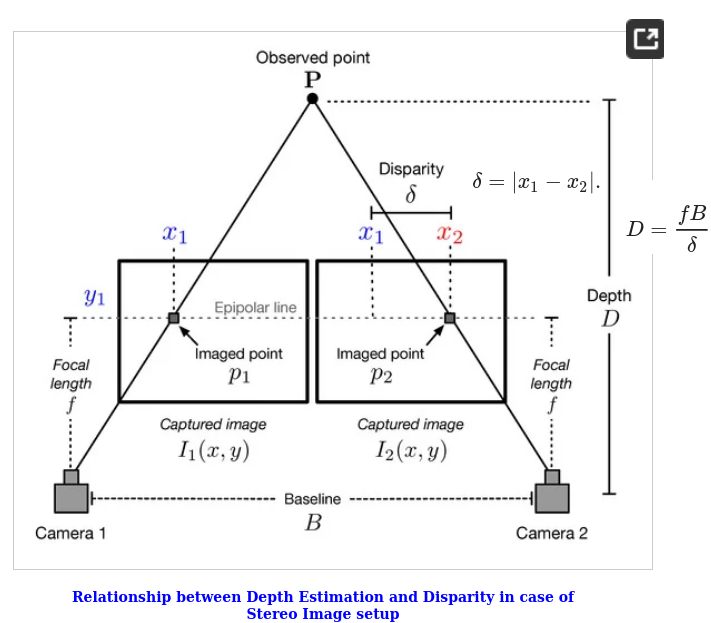
\includegraphics[width=\textwidth]{images/methodology/depth_estimation_a.png}
        \caption{}
        \label{fig:depth_estimation_a}
    \end{subfigure}
    \hfill
    \begin{subfigure}[b]{0.18\textwidth}
        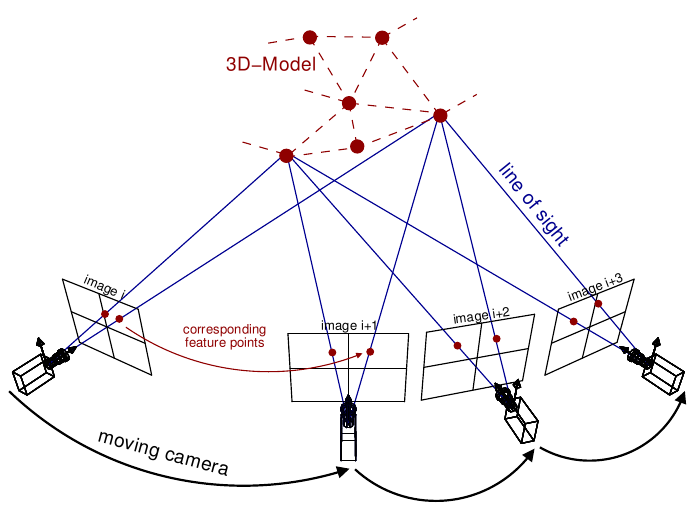
\includegraphics[width=\textwidth]{images/methodology/depth_estimation_b.png}
        \caption{}
        \label{fig:depth_estimation_b}
    \end{subfigure}
    \hfill
    \begin{subfigure}[b]{0.18\textwidth}
        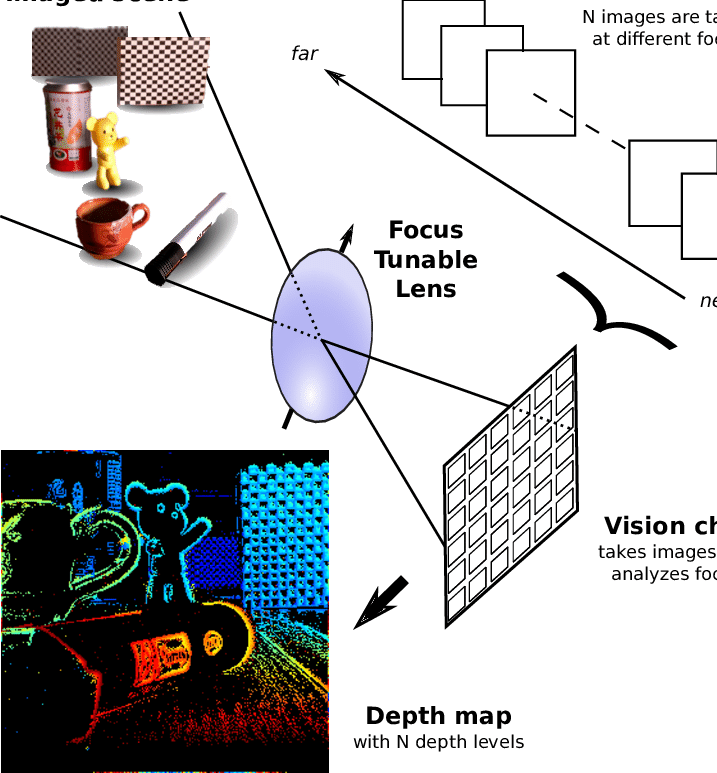
\includegraphics[width=\textwidth]{images/methodology/depth_estimation_c.png}
        \caption{}
        \label{fig:depth_estimation_c}
    \end{subfigure}
    \hfill
    \begin{subfigure}[b]{0.18\textwidth}
        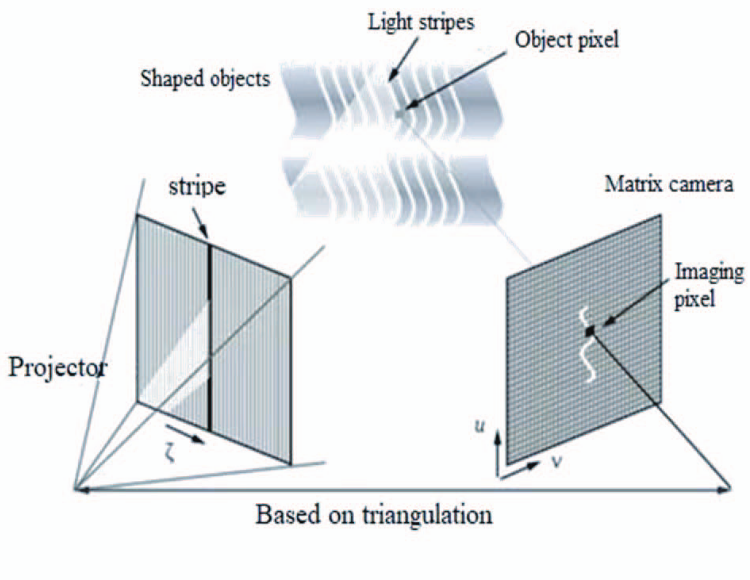
\includegraphics[width=\textwidth]{images/methodology/depth_estimation_d.png}
        \caption{}
        \label{fig:depth_estimation_d}
    \end{subfigure}
    \hfill
    \begin{subfigure}[b]{0.18\textwidth}
        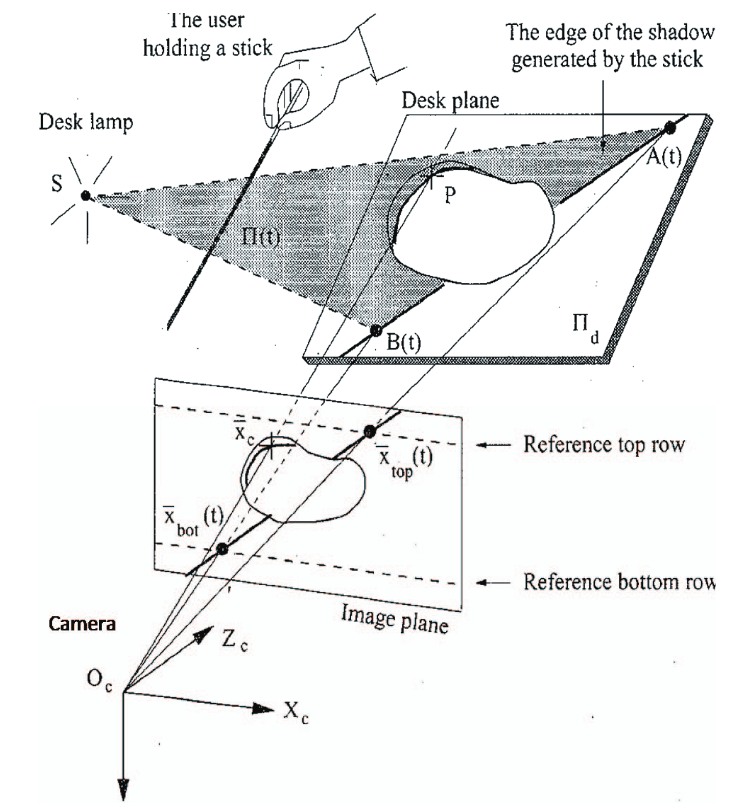
\includegraphics[width=\textwidth]{images/methodology/depth_estimation_e.png}
        \caption{}
        \label{fig:depth_estimation_e}
    \end{subfigure}

    \caption{Traditional depth estimation techniques: (a) stereo-depth, (b) structure from motion, (c) depth-from-defocus, (d) photometric-depth, and (e) shape from shading.}
    \label{fig:depth_estimation}
\end{figure}

With the continuous development of deep learning technologies, depth estimation and 3D reconstruction methods based on these approaches are constantly updated. They have become a powerful choice for monocular depth estimation as they offer high reconstruction accuracy and computational efficiency. However, a common limitation of such models is their dependency on training data as performance tends to decrease if the target image is not consistent with the learning database.

This is where Depth-Pro \cite{depth-pro} comes into as it is 'a foundation model for zero-shot metric monocular depth estimation'. Trained on a large and diverse dataset, Depth-Pro generalizes well across multiple real-world scenarios and achieves state-of-the-art performance without requiring fine-tuning. For this thesis, Depth-Pro has been chosen as the monocular depth estimation model to generate depth maps for annotation purposes.

\begin{figure}[h!]
    \centering
    % Row labels
    \setlength{\tabcolsep}{1pt}  % Reduce column padding
    \renewcommand{\arraystretch}{0.5}
    \begin{tabular}{c c c c c c c c}
        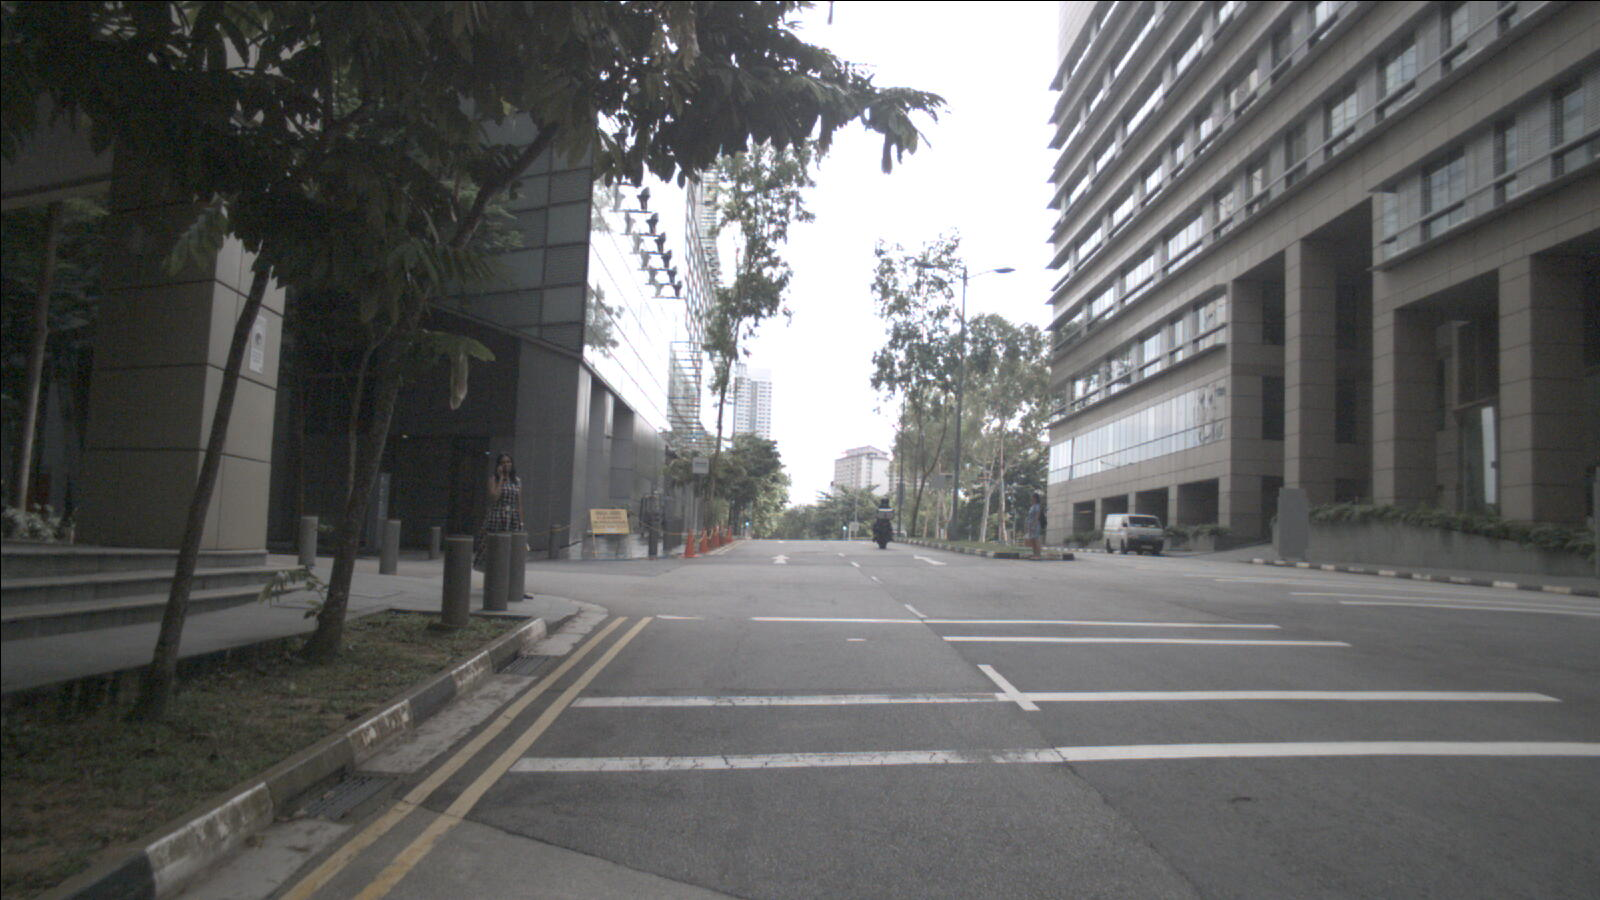
\includegraphics[width=0.12\textwidth]{images/methodology/raw/original_image_0.png} & 
        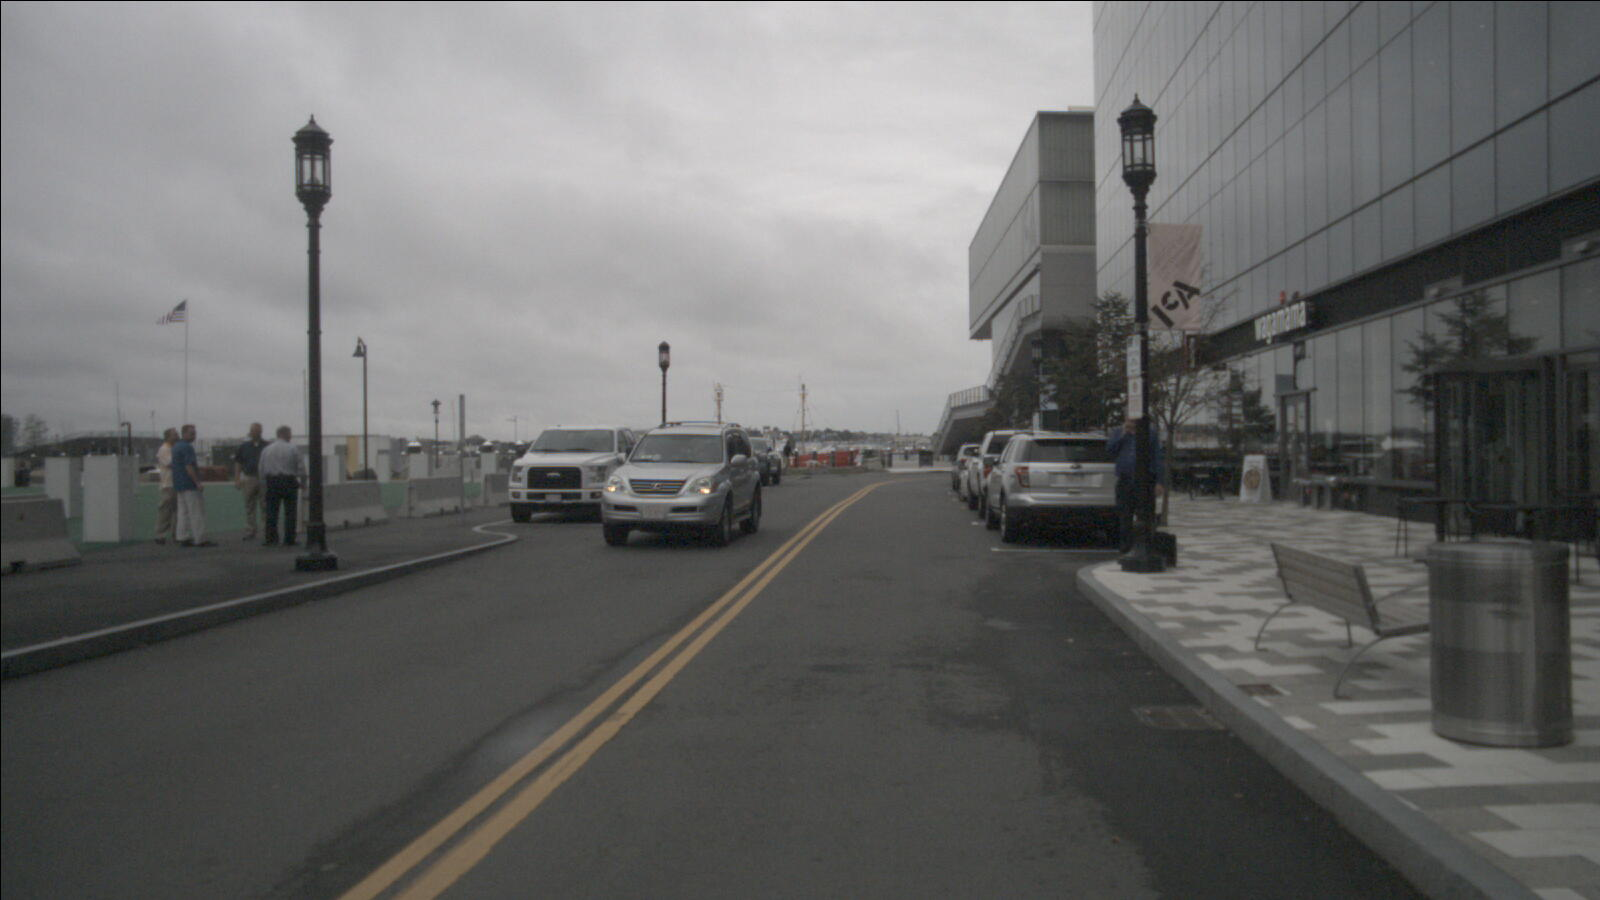
\includegraphics[width=0.12\textwidth]{images/methodology/raw/original_image_1.png} & 
        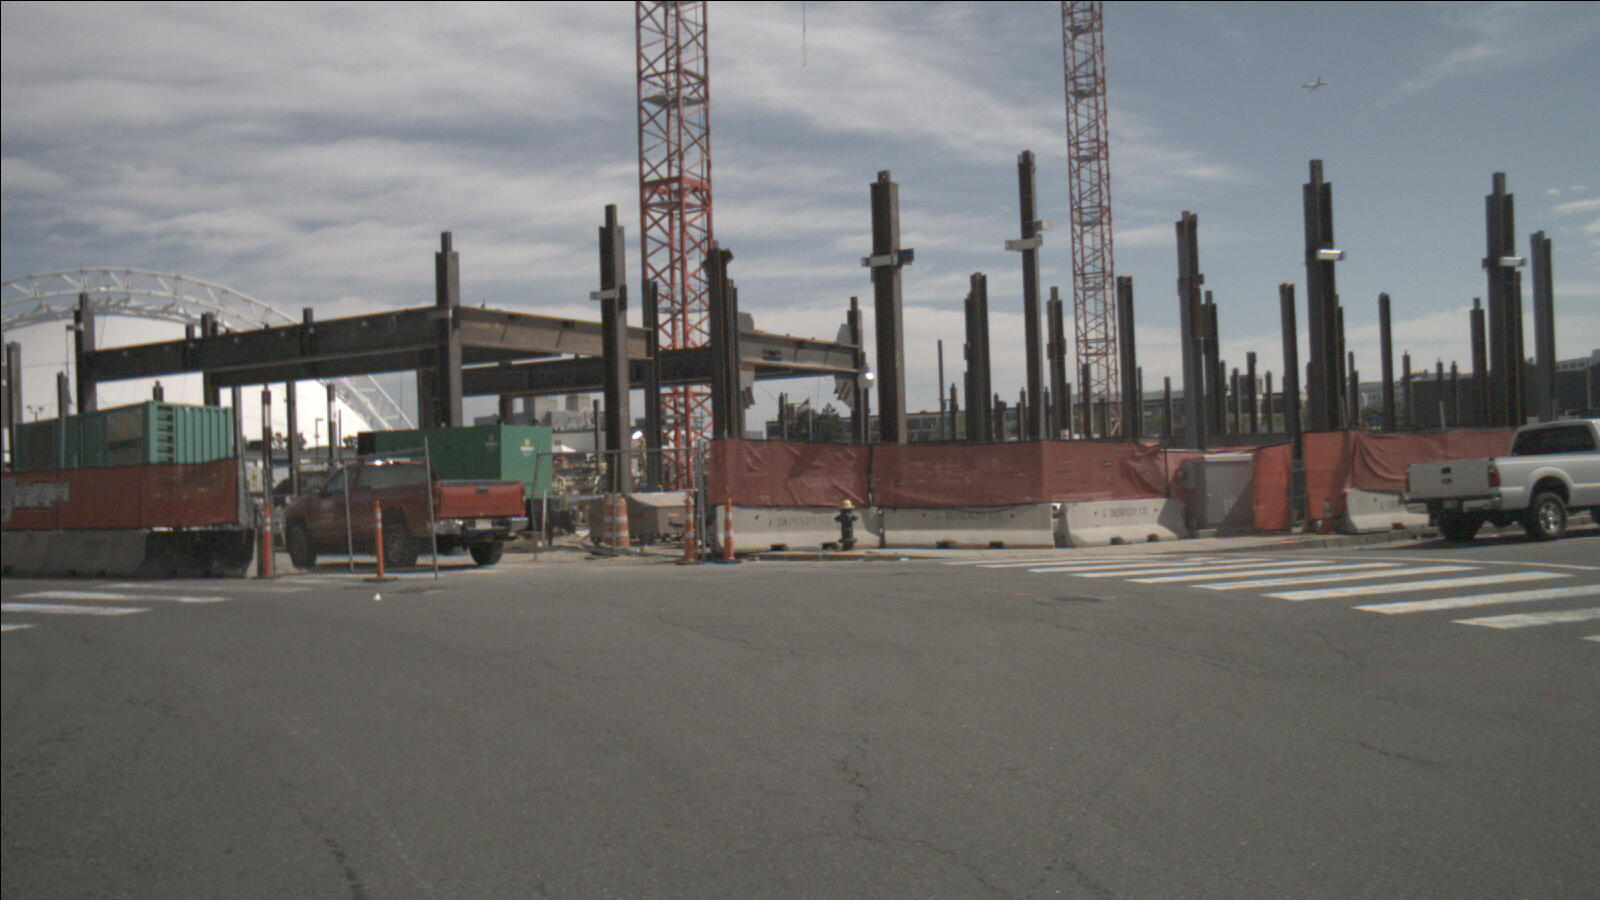
\includegraphics[width=0.12\textwidth]{images/methodology/raw/original_image_2.png} &
        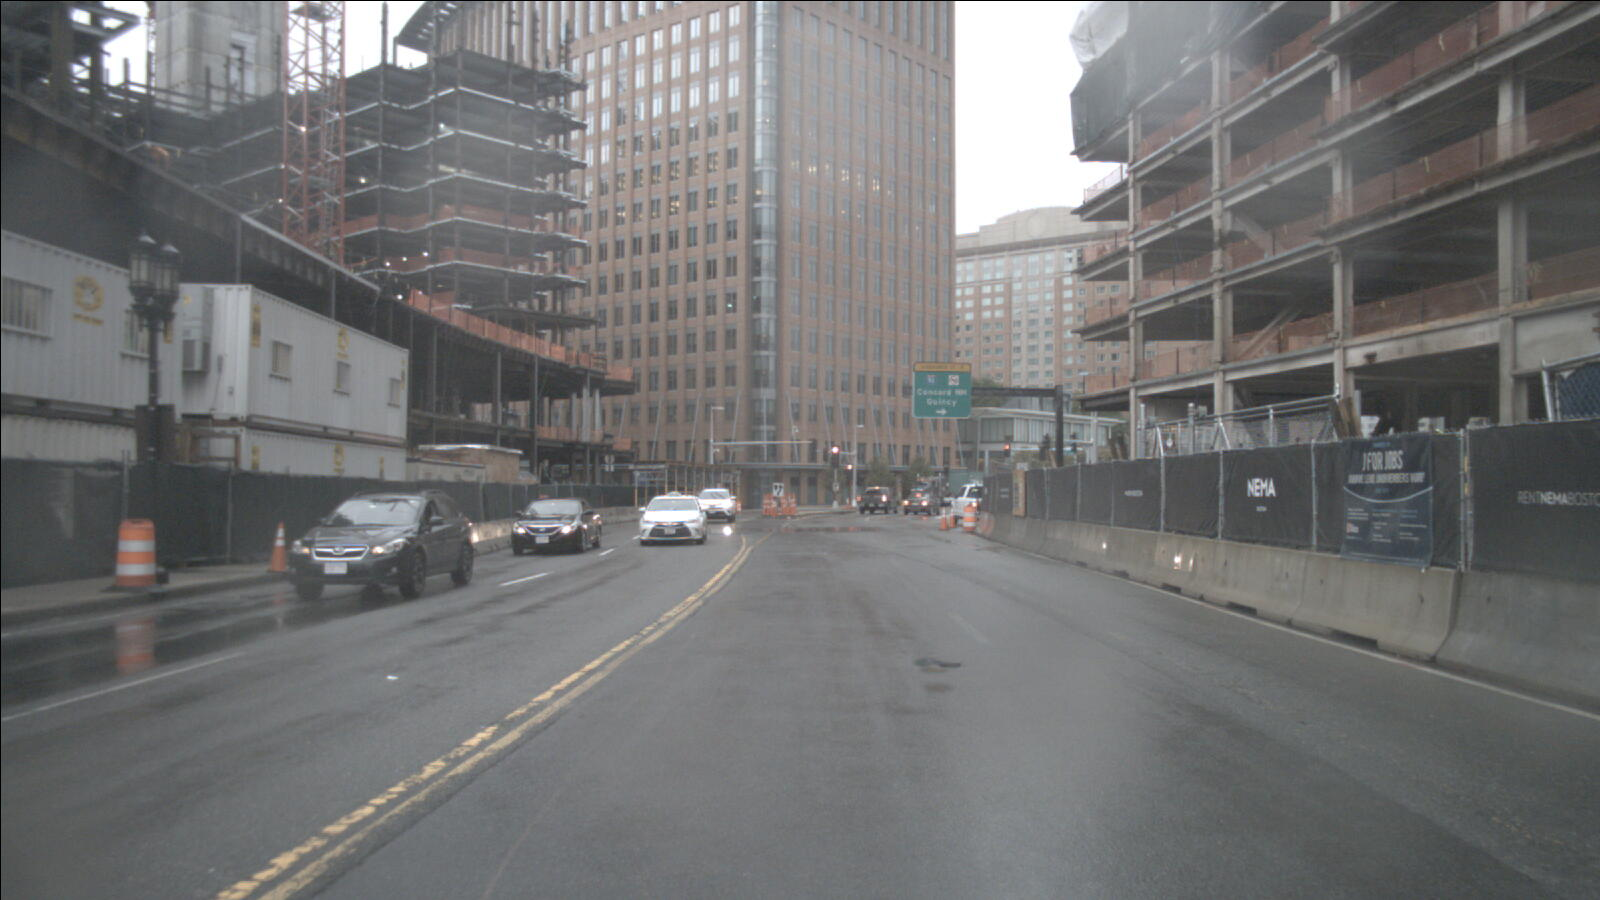
\includegraphics[width=0.12\textwidth]{images/methodology/raw/original_image_3.png} &
        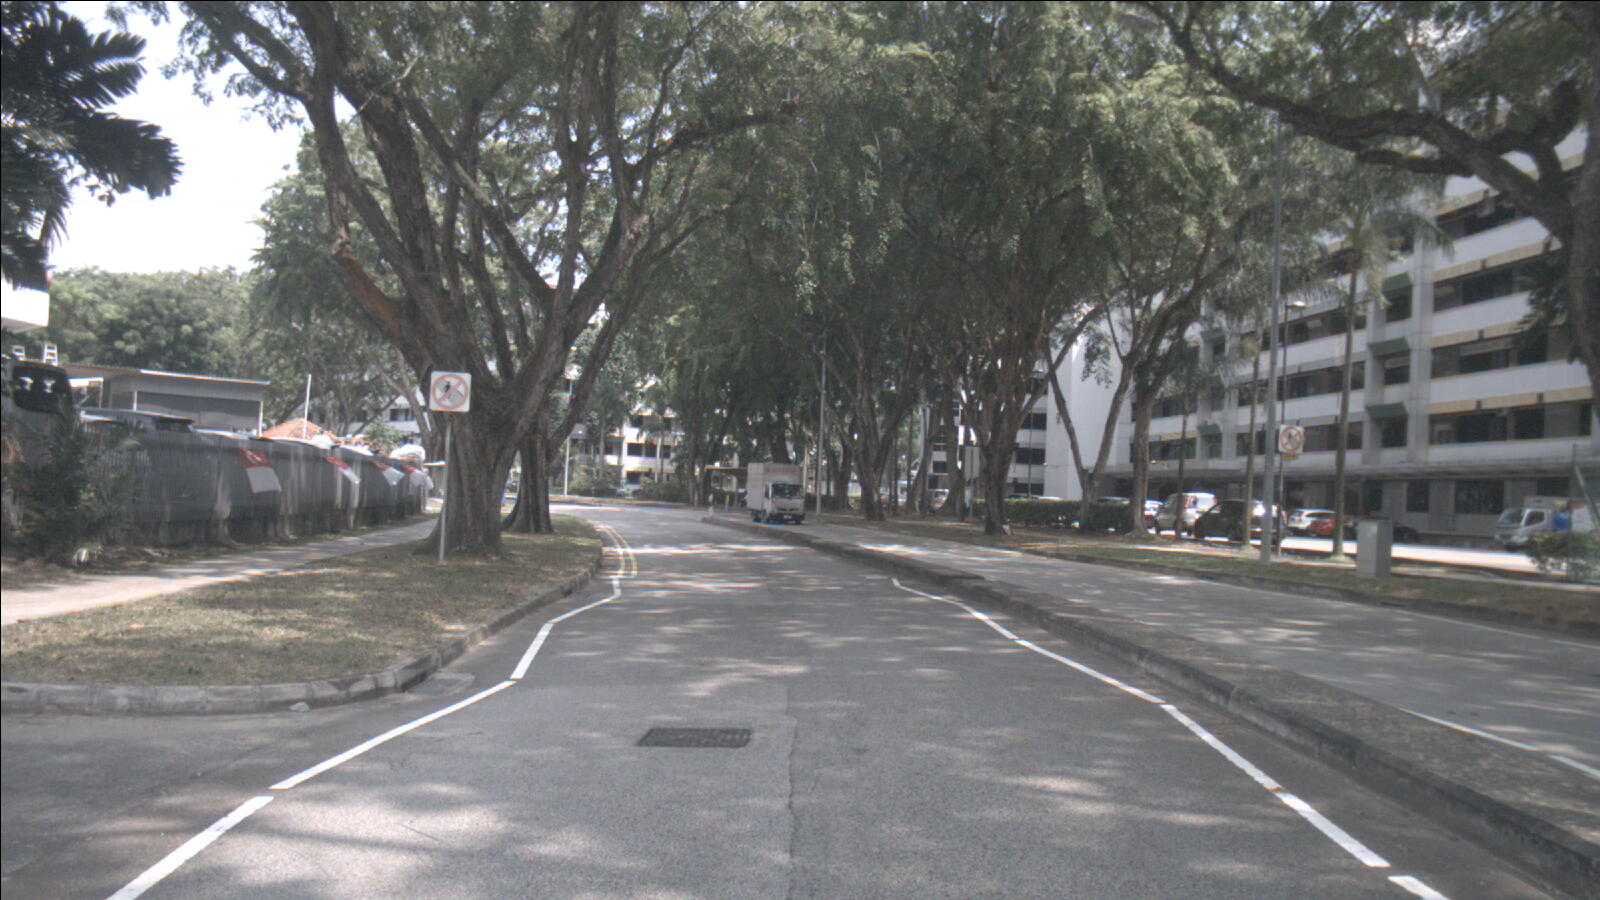
\includegraphics[width=0.12\textwidth]{images/methodology/raw/original_image_4.png} &   
        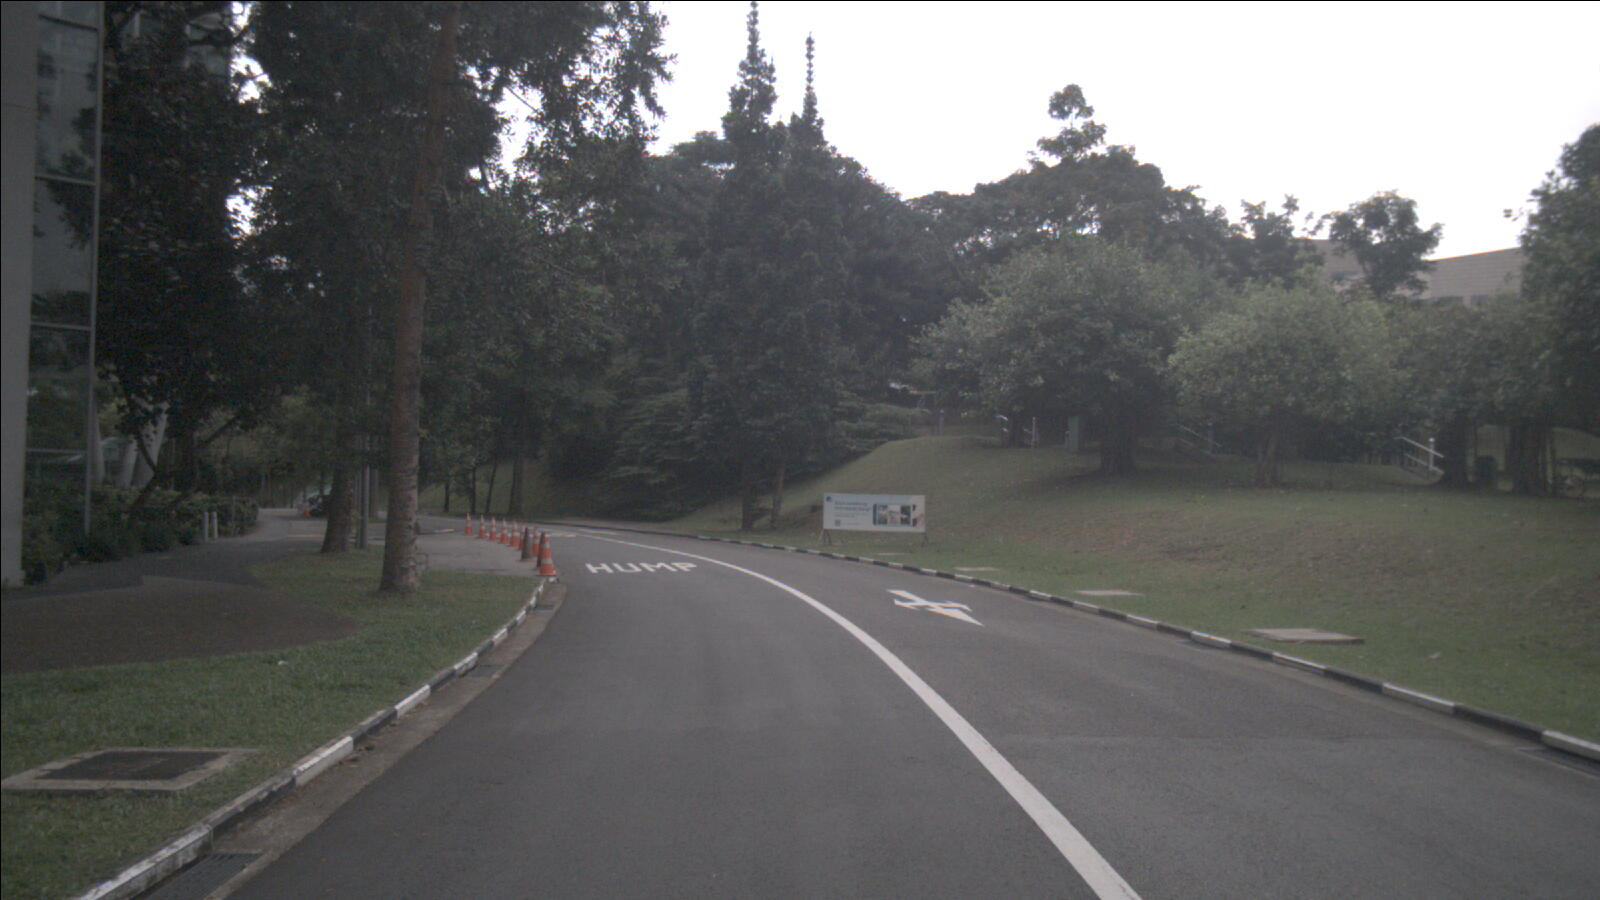
\includegraphics[width=0.12\textwidth]{images/methodology/raw/original_image_5.png} & 
        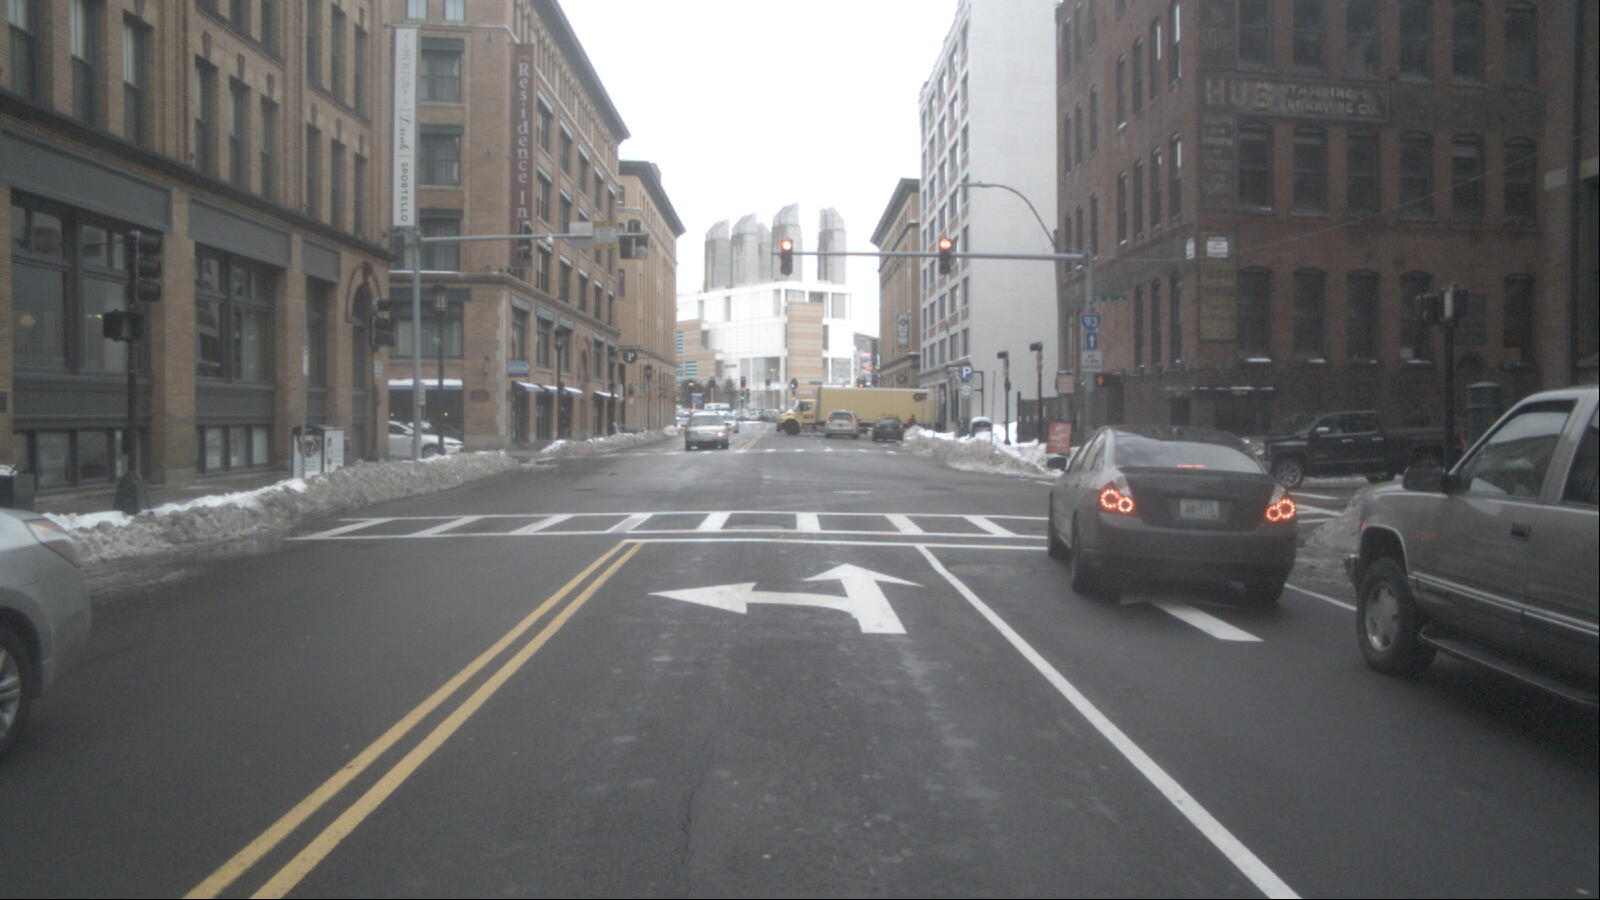
\includegraphics[width=0.12\textwidth]{images/methodology/raw/original_image_6.png} &
        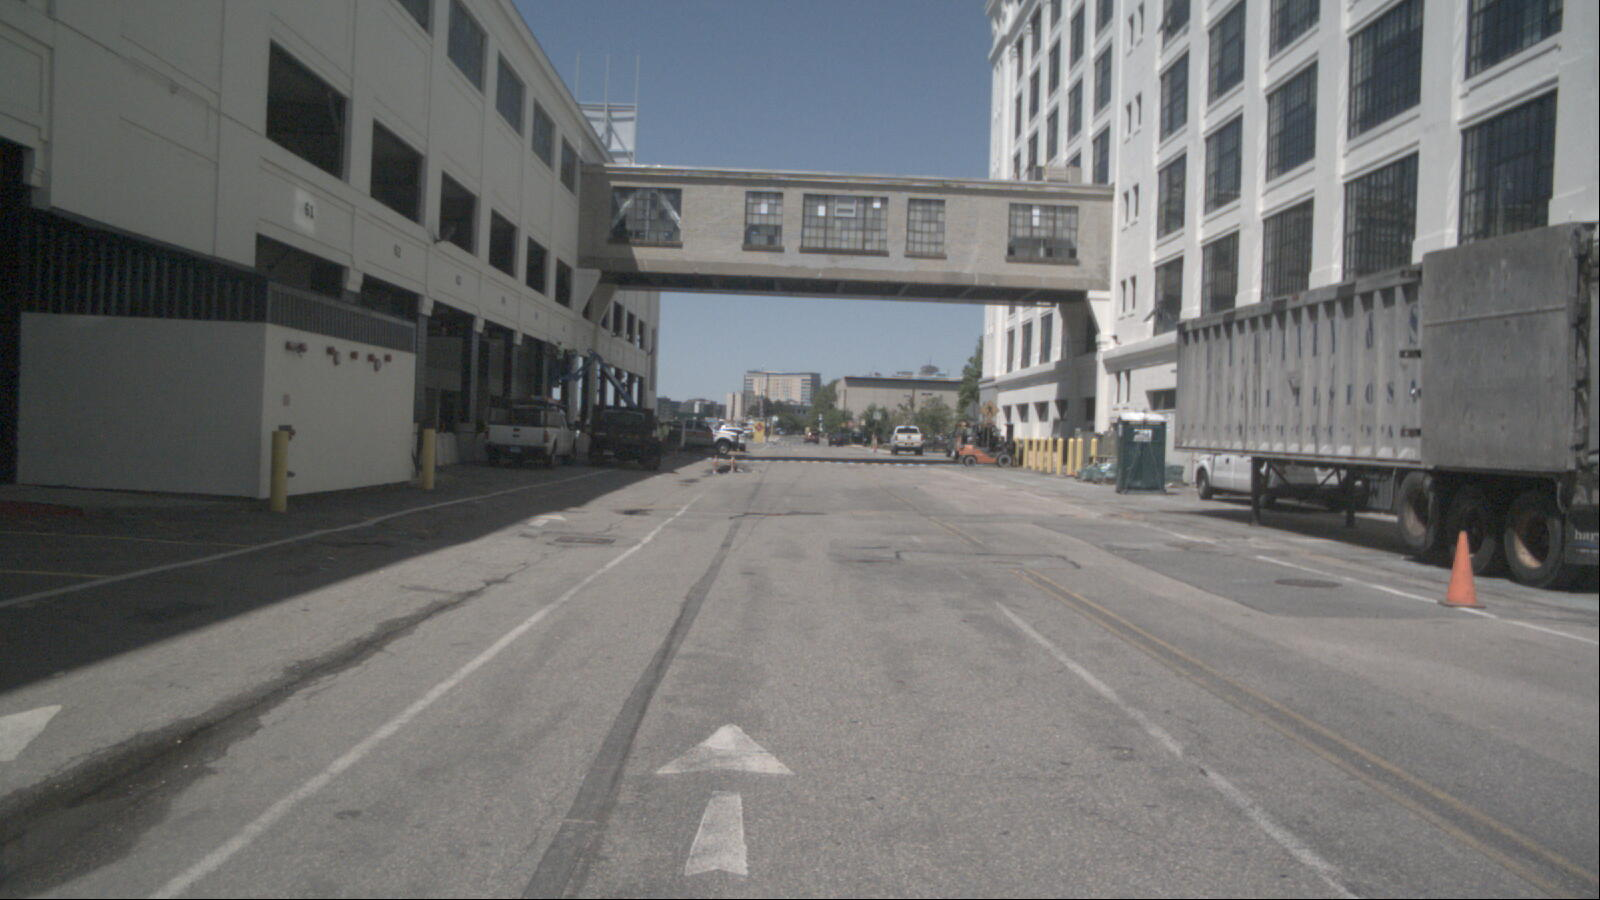
\includegraphics[width=0.12\textwidth]{images/methodology/raw/original_image_7.png} \\

        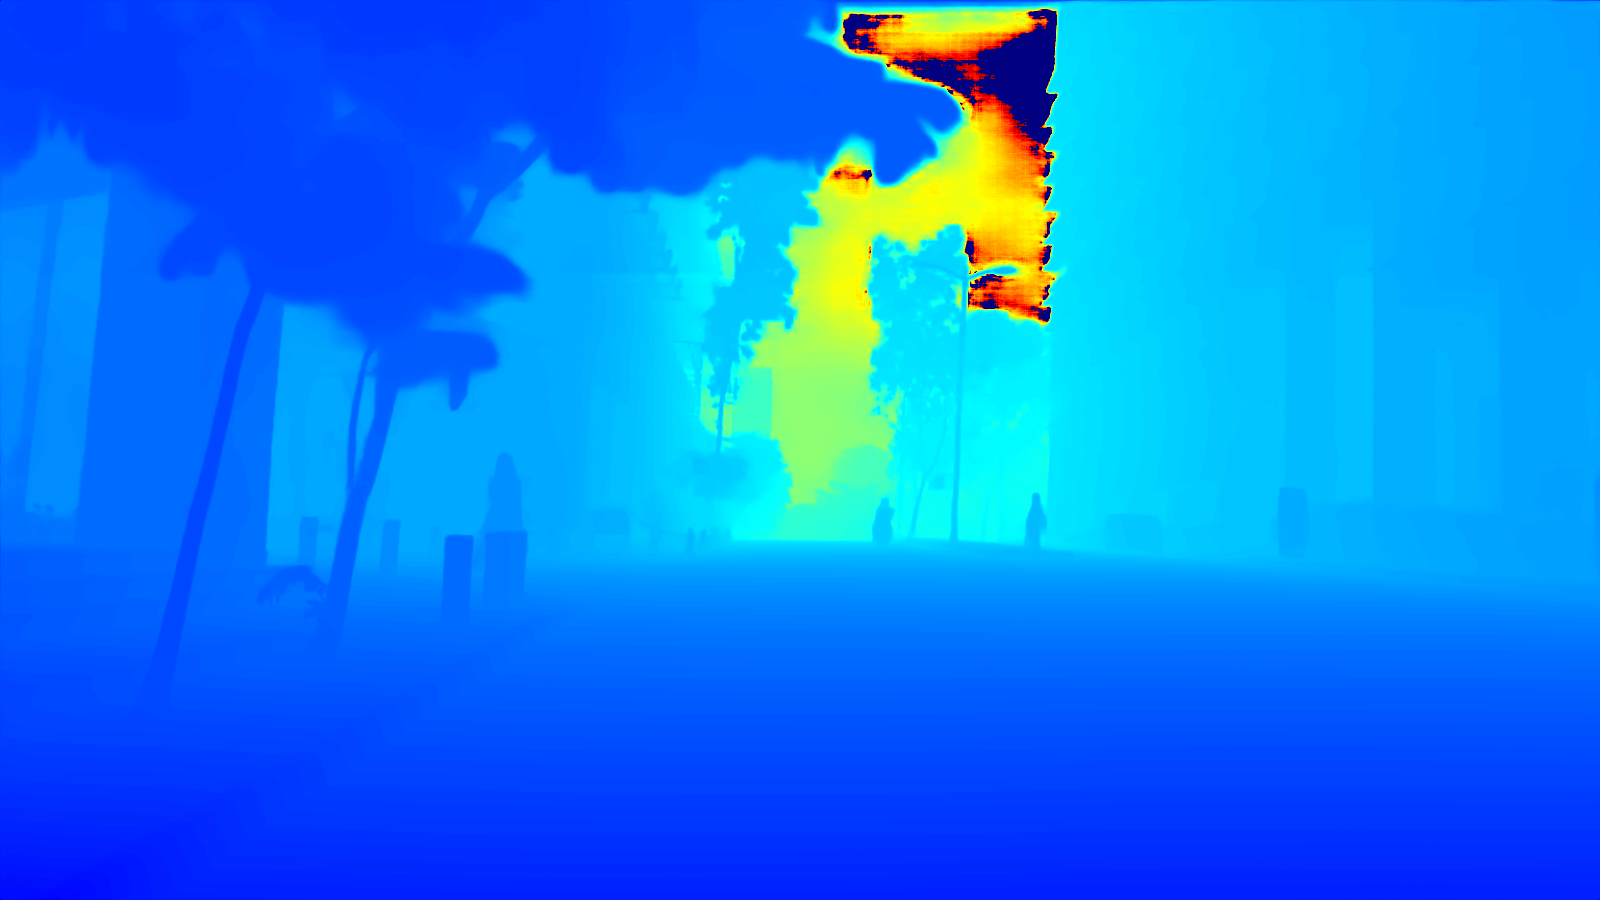
\includegraphics[width=0.12\textwidth]{images/methodology/depth_images/colored_depth_map_0.png} & 
        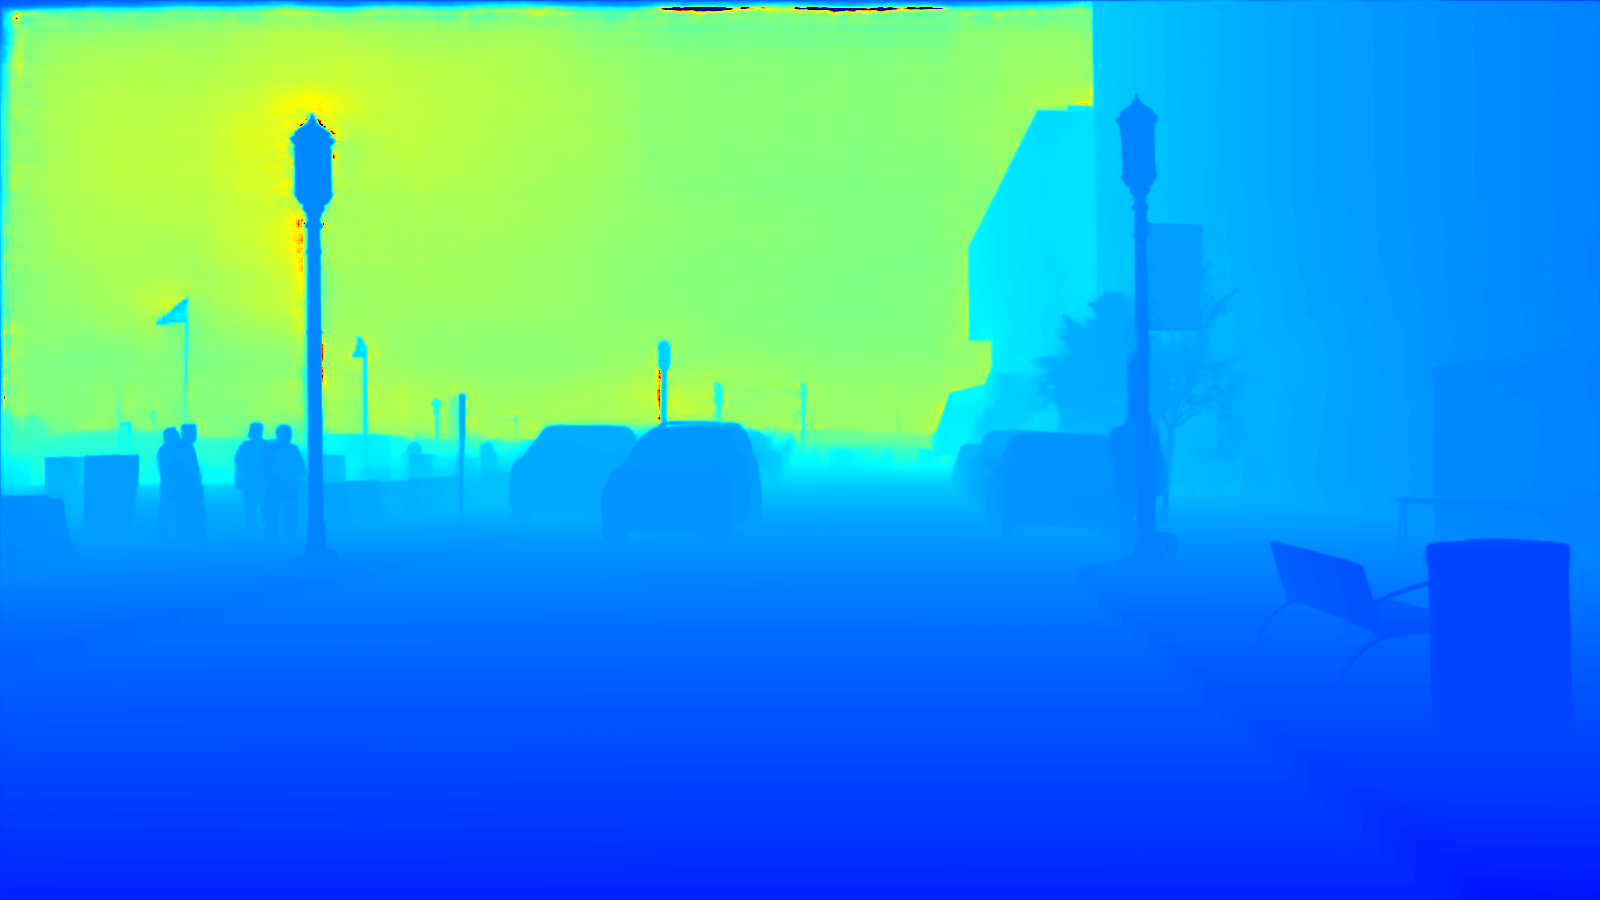
\includegraphics[width=0.12\textwidth]{images/methodology/depth_images/colored_depth_map_1.png} & 
        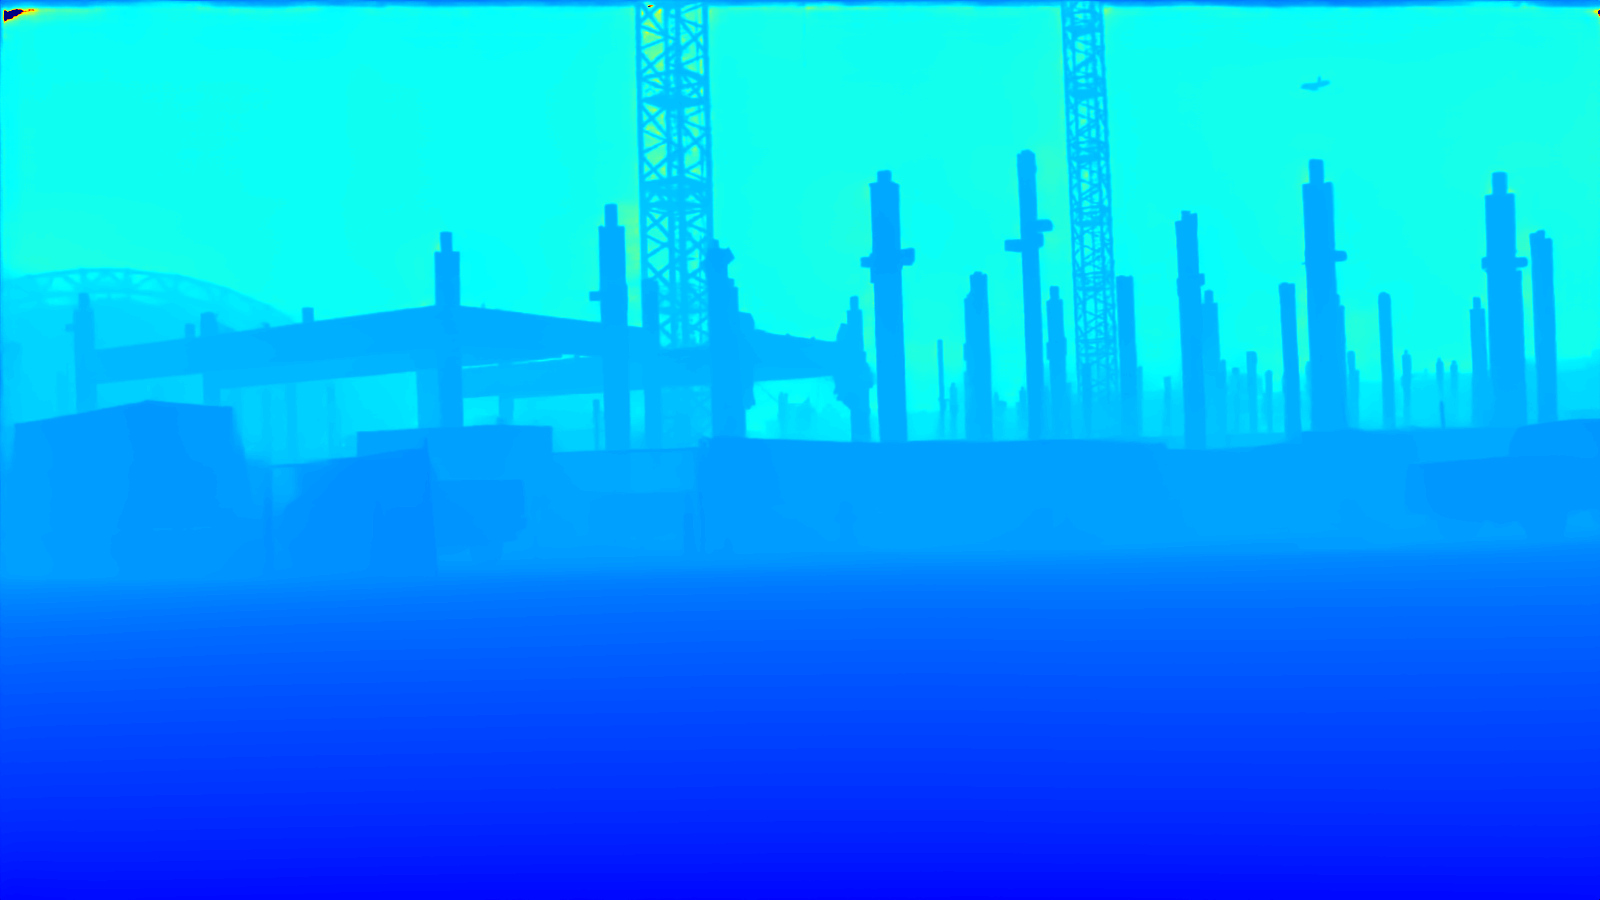
\includegraphics[width=0.12\textwidth]{images/methodology/depth_images/colored_depth_map_2.png} &
        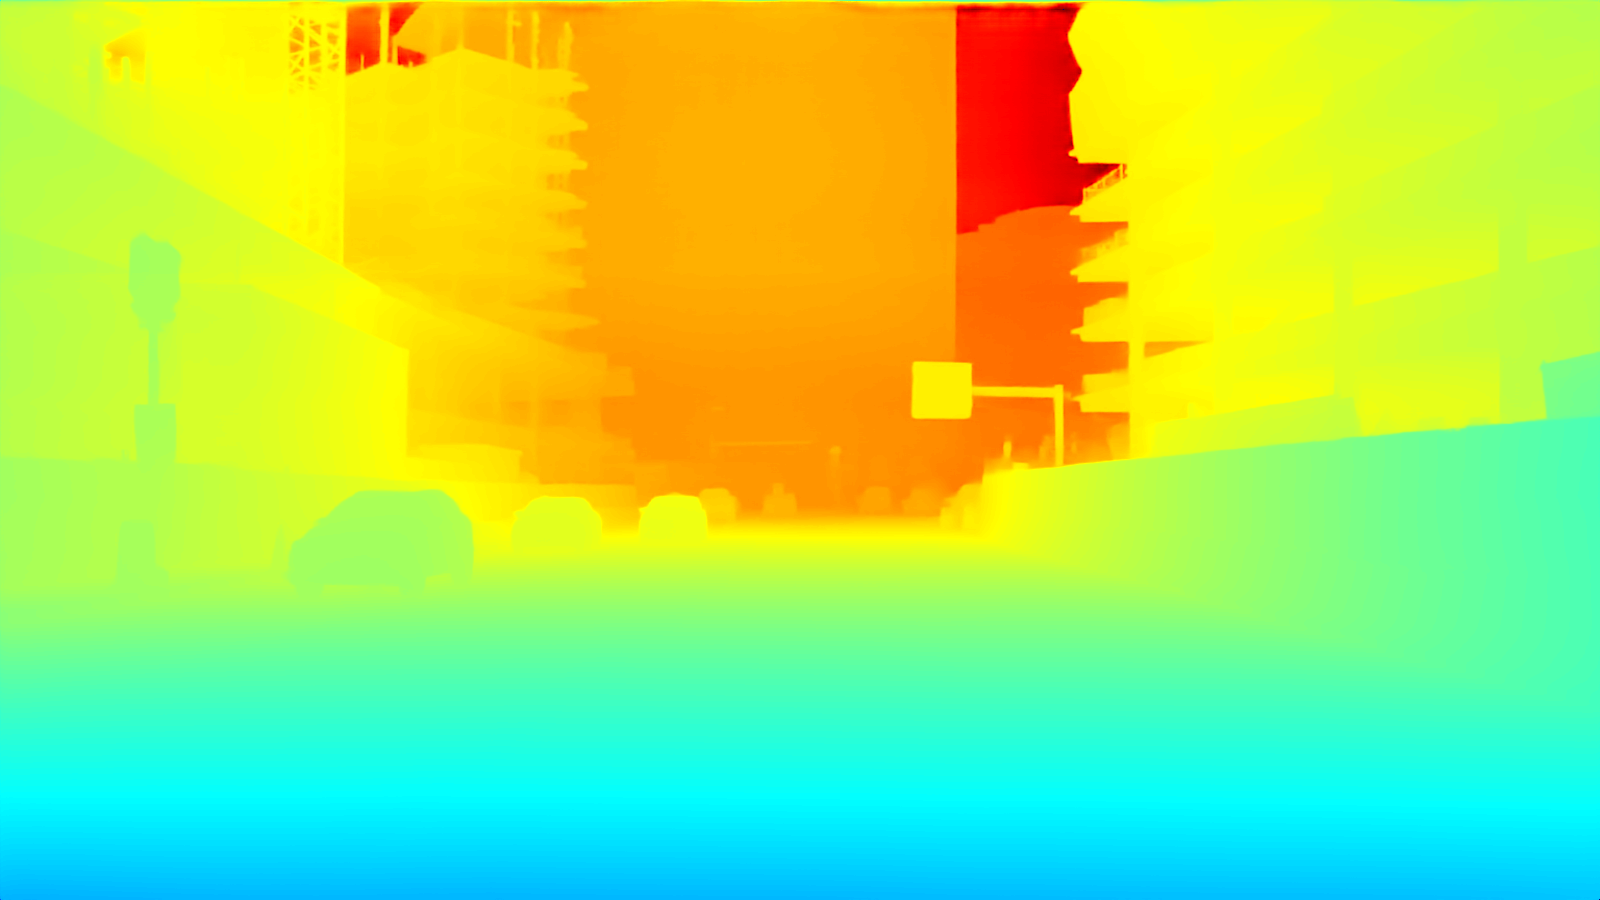
\includegraphics[width=0.12\textwidth]{images/methodology/depth_images/colored_depth_map_3.png} &
        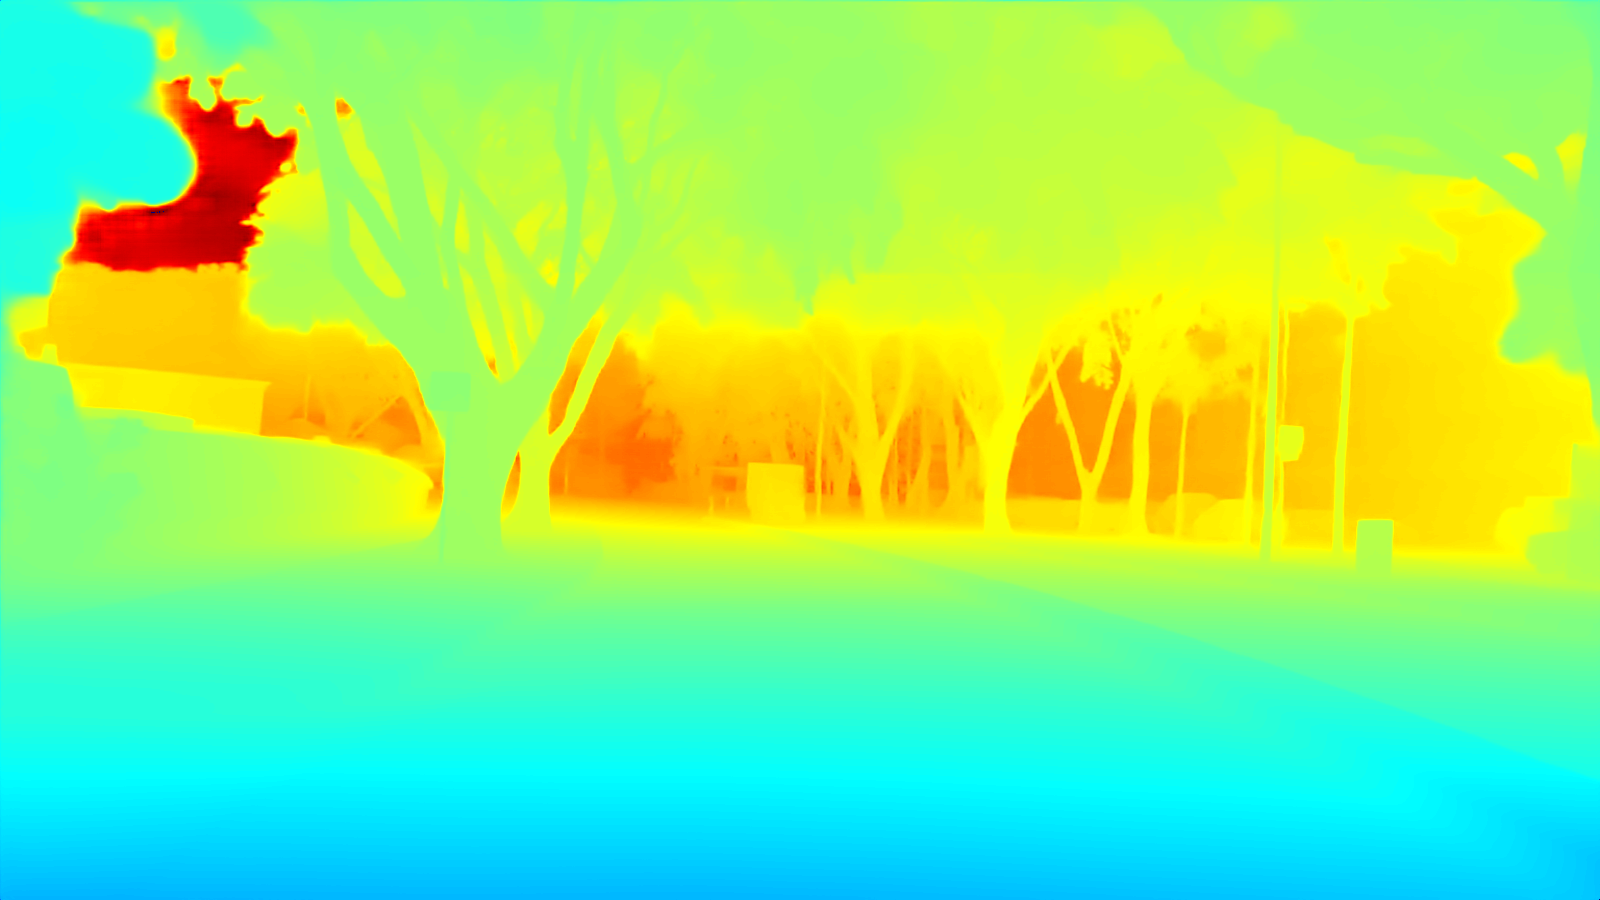
\includegraphics[width=0.12\textwidth]{images/methodology/depth_images/colored_depth_map_4.png} &   
        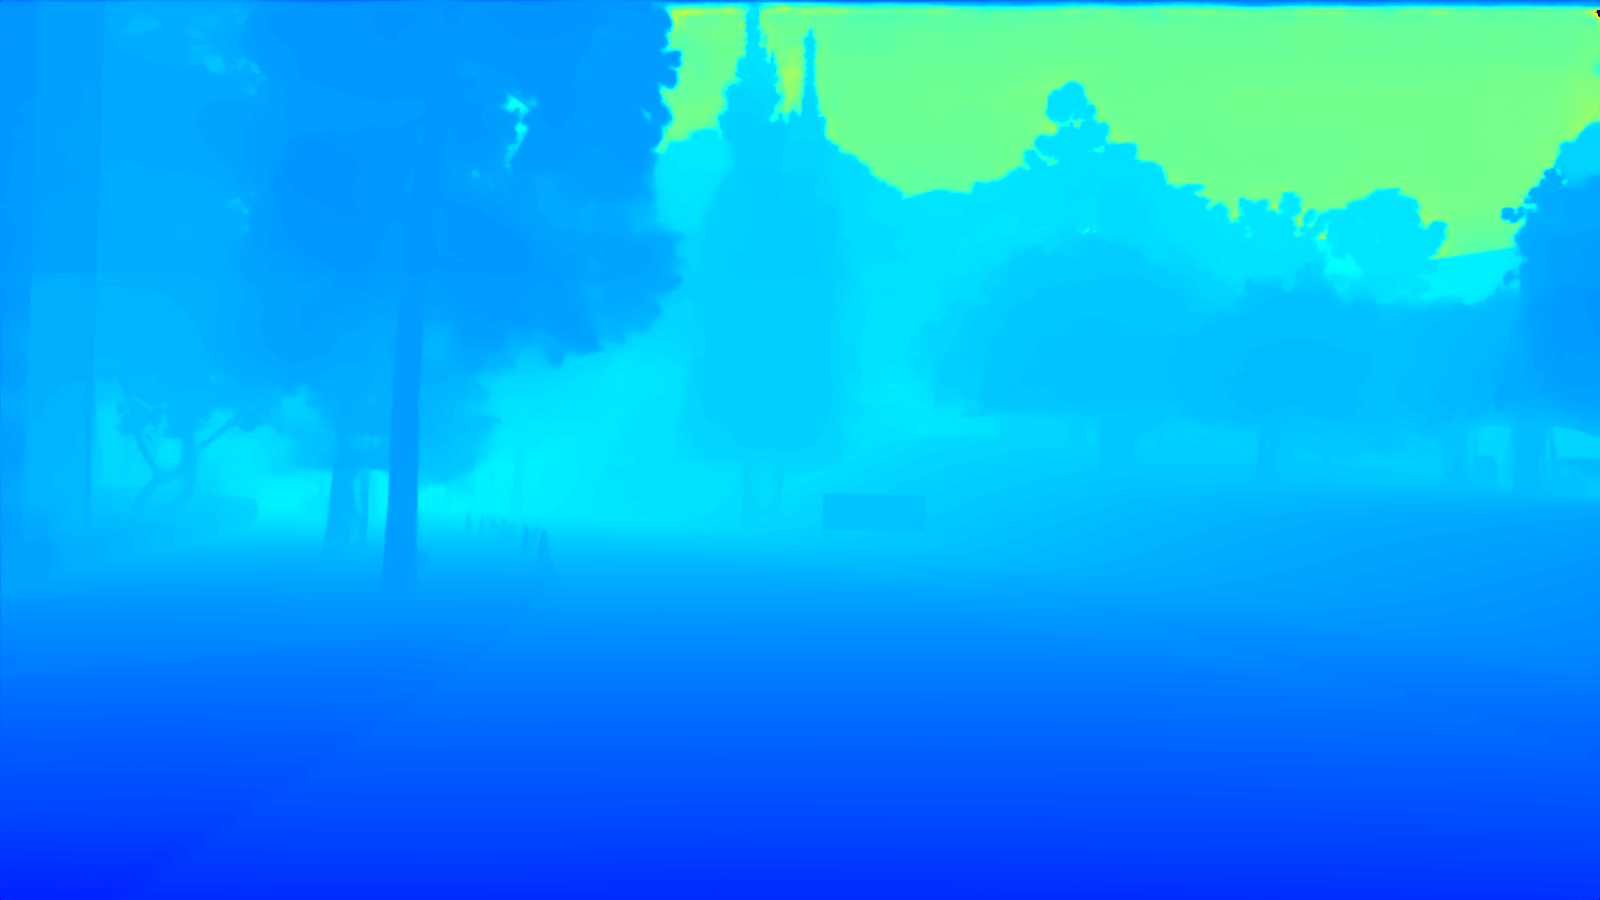
\includegraphics[width=0.12\textwidth]{images/methodology/depth_images/colored_depth_map_5.png} & 
        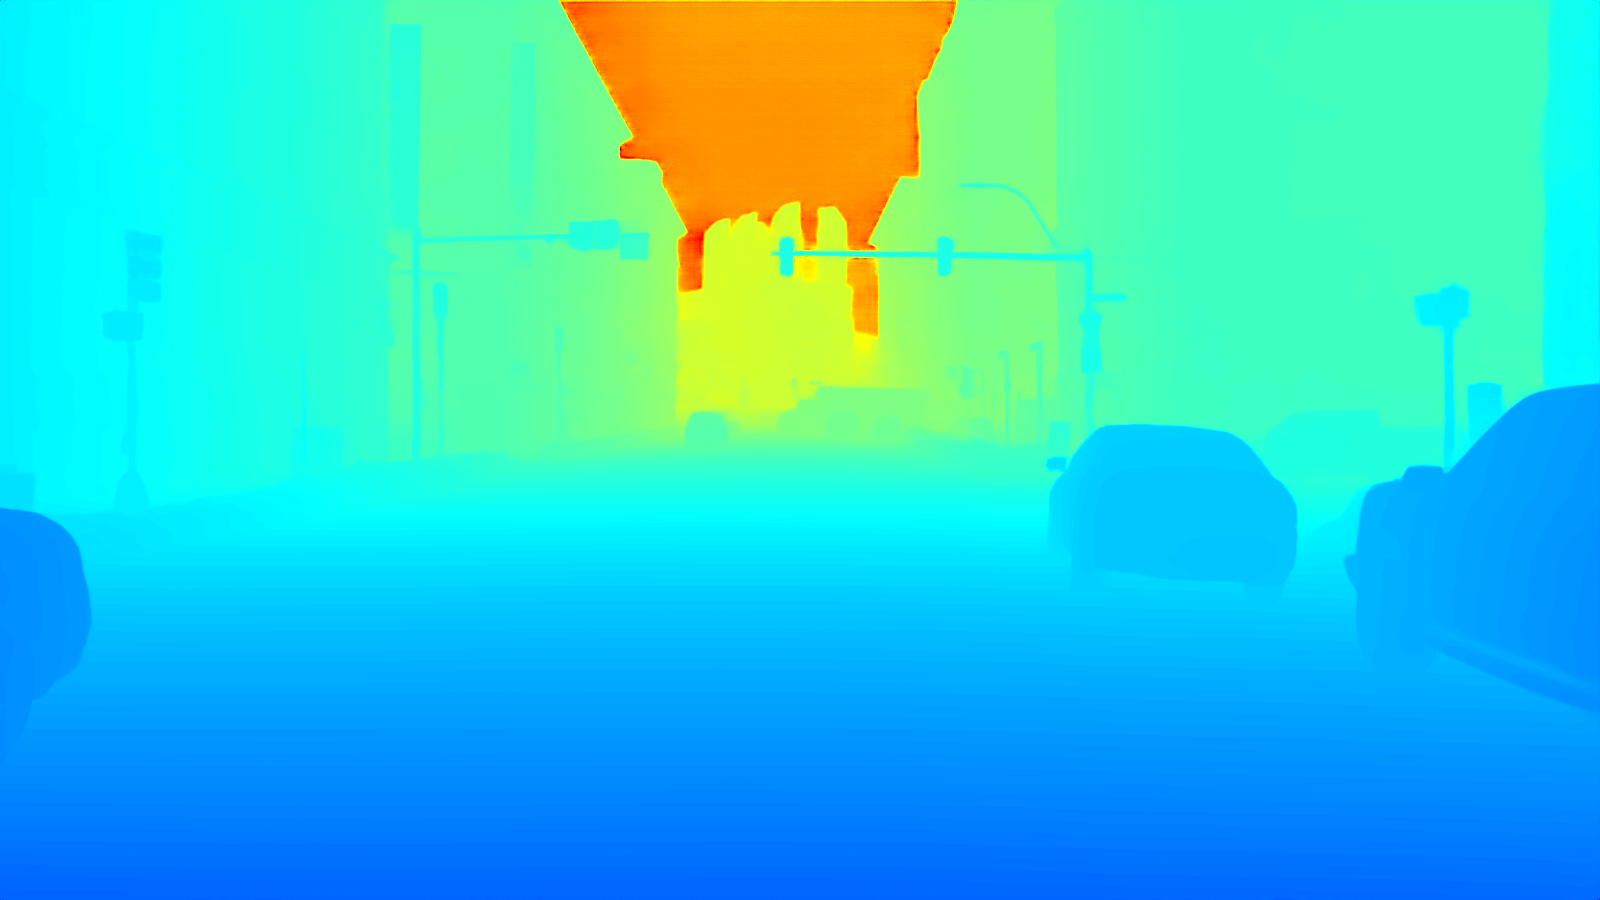
\includegraphics[width=0.12\textwidth]{images/methodology/depth_images/colored_depth_map_6.png} &
        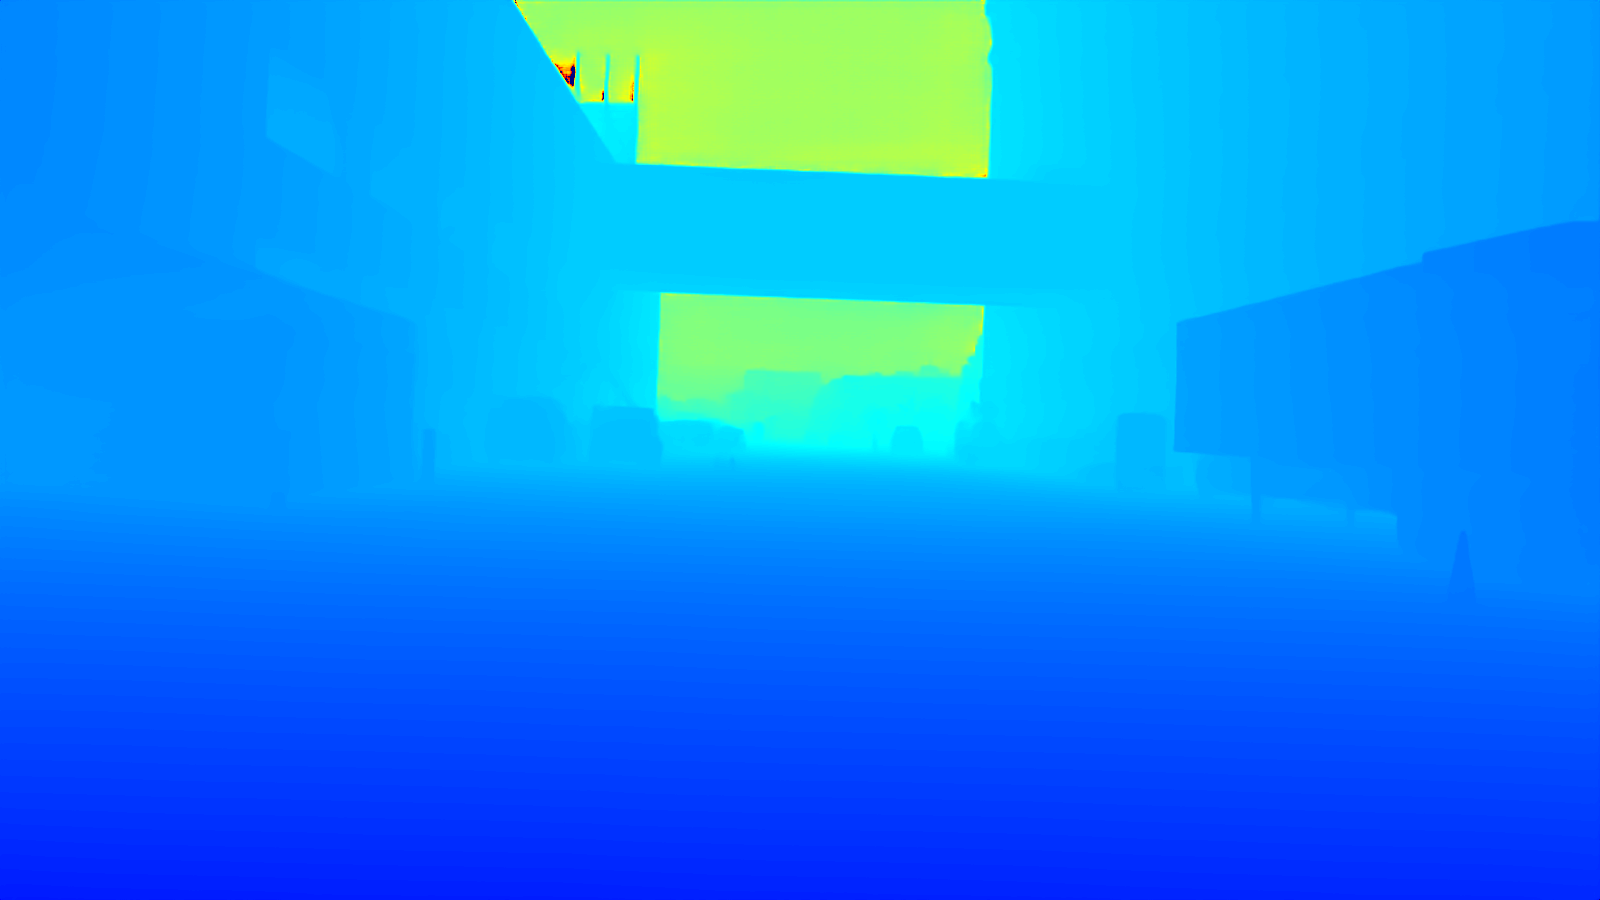
\includegraphics[width=0.12\textwidth]{images/methodology/depth_images/colored_depth_map_7.png} \\
    \end{tabular}    
    \caption{Depth maps of BEVDataset 'mini' estimated with Depth-Pro model.}
    \label{fig:depth_images}
\end{figure}

\subsubsection{Scene PCD}
When an image is captured, the 3D geometry of the scene is projected onto a 2D representation, which is then rasterized into the pixel space of the image. This transformation from 3D world coordinates to 2D image coordinates is known as the \emph{camera projection process}. In its simplest form, this is described by the \emph{pinhole camera model}, illustrated in Figure~\ref{fig:pinhole_model}. In this setup, $\mathbf{O}_w$ represents the world coordinate frame, $\mathbf{F}_c$ denotes the camera coordinate frame (typically located at the camera's optical center or pinhole), and $\mathbf{F}_i$ defines the 2D image plane.

\begin{figure}[h!]
    \centering
    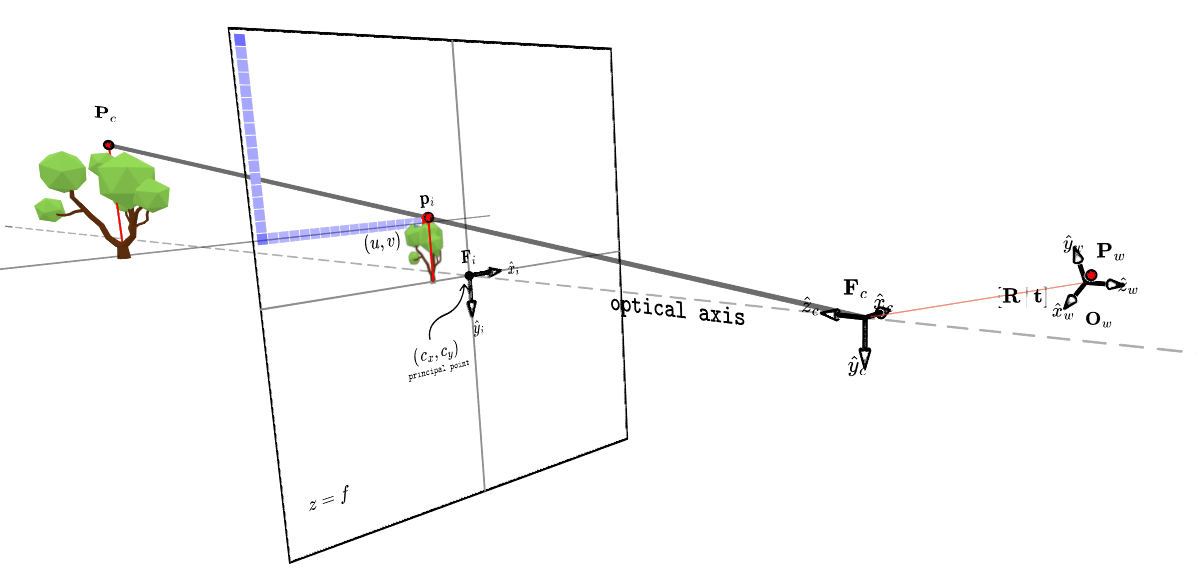
\includegraphics[width=0.5\linewidth]{images/methodology/pinhole_model/pinhole_model_2.png}
    \caption{Ideal perspective camera model.}
    \label{fig:pinhole_model}
\end{figure}

Starting with a 3D point expressed in world coordinates, $\mathbf{P}_w = \left(x_w, y_w, z_w\right)^\top$, the point can be transformed int the camera coordinate frame using a rotation matrix $\mathbf{R}$ and a translation vector $\mathbf{t}$. These are known as camera's extrinsic parameters and are commonly combined into a single homogeneous transformation matrix denoted as $\left[\mathbf{R} \,|\, \mathbf{t}\right]$.

\begin{align}
    \tilde{\mathbf{P}}_c 
    &=
    \begin{pmatrix}
        x_c \\
        y_c \\
        z_c \\
        1
    \end{pmatrix}
    =
    \begin{pmatrix}
        r_{11} & r_{12} & r_{13} & t_x \\
        r_{21} & r_{22} & r_{23} & t_y \\
        r_{31} & r_{32} & r_{33} & t_z \\
        0 & 0 & 0 & 1
    \end{pmatrix}
    \begin{pmatrix}
        x_w \\
        y_w \\
        z_w \\
        1
    \end{pmatrix}
    =
    \left[ \mathbf{R} \,|\, \mathbf{t} \right] \tilde{\mathbf{P}}_w 
\end{align}

Once the point is expressed in the camera coordinate frame $\mathbf{F}_c$, it is projected onto the image plane $\mathbf{F}_i$ using the intrinsic parameters of the camera, which describe how the 3D geometry of the scene is mapped to the 2D image sensor. Under the pinhole camera model, this projection involves a perspective division (to normalize the coordinates) followed by a transformation using the intrinsic matrix $\mathbf{K}$, which encodes the focal lengths and maps the continuous 2D space to the discrete pixel grid of the digital camera, while also considering the sensor's displacement of the principal point $(c_x, c_y)$. The final pixel coordinates can be computed as:

\begin{align}
    \tilde{\mathbf{p}_i}
    = \left(u, v, 1\right)^\top
    = \mathbf{K} \cdot \frac{1}{z_c} \tilde{\mathbf{P}}_c
\end{align}

where $\mathbf{K}$ is the intrinsic calibration matrix, typically given by:

\begin{align}
    \mathbf{K} =
    \begin{pmatrix}
        f_x & 0 & c_x \\
        0 & f_y & c_y \\
        0 & 0 & 1
    \end{pmatrix}
\end{align}

Here, $f_x$ and $f_y$ are the focal lengths in pixel units along the $\hat{x}_i$ and $\hat{y}_i$ axes.

However, the images used in this thesis were captured using lens-based cameras, which introduce radial and tangential distortions. These distortions are taken into account by rectifying the normalized 3D coordinates in the camera frame before applying the camera's intrinsic matrix $\mathbf{K}$.

Despite this, the objective of this module is to perform the inverse process: reconstructing the 3D structure of the scene from 2D image pixels. This process is known as \textit{reprojection}, and it has the challenging task of recovering the third spatial dimension, which is inherently lost during the image acquisition process. To address this, a depth map $D_{h \times w}$ is estimated (see Section~\ref{sec:depth_estimation}), where $h$ and $w$ correspond to the height and width of the image, respectively. It is also assumed that the camera parameters (intrinsics and extrinsics) are known.

The approach employed for this task is detailed in Algorithm~\ref{algorithm:scene_pcd_hloop} where for each pixel column in the vertical range $\left[0, 1, \dots, h{-}1 \right]$, a 3D ray is projected from the camera center and then intersected with the depth value estimated for that pixel. The final result is a dense 3D point cloud which can be seen in Figure~\ref{fig:raw_pointcloud}.

\begin{algorithm}
    \caption{Pointcloud calculation}
    \label{algorithm:scene_pcd_hloop}
    \footnotesize

    \begin{algorithmic}[1]
        \State \textbf{Input:} Depth map $D_{\left[h \times w\right]}$, camera intrinsics $K$ 
        \State \textbf{Output:} Pointcloud $P^{raw}_{\left[3 \times h \times w\right]}$
        
        \State Initialize $P_{\left[3 \times h \times w\right]} \gets \mathbf{0}$

        \For{$i \text{ in } \left[0, 1, \dots, h-1\right]$}
            \State $pix\_coords_{3 \times w} \gets \begin{bmatrix} \text{0:w-1} & \mathbf{i}_w & \mathbf{1}_w \end{bmatrix}$
            \State $cam\_rays_{3 \times w} \gets \texttt{UnDistord} \left( \texttt{Normalize} \left( K^{-1} \cdot pix\_coords \right)\right)$
            
            \State $P^{raw}[:, i, :] \gets cam\_rays[2, :] \cdot D[i, :]$  \Comment{Update the $i$-th row of $P$. The ray's z-value is the depth}
        \EndFor
        
        \State \Return $P^{raw}$
    \end{algorithmic}
\end{algorithm}
\begin{figure}[h!]
    \centering
    \begin{subfigure}[b]{0.45\textwidth}
        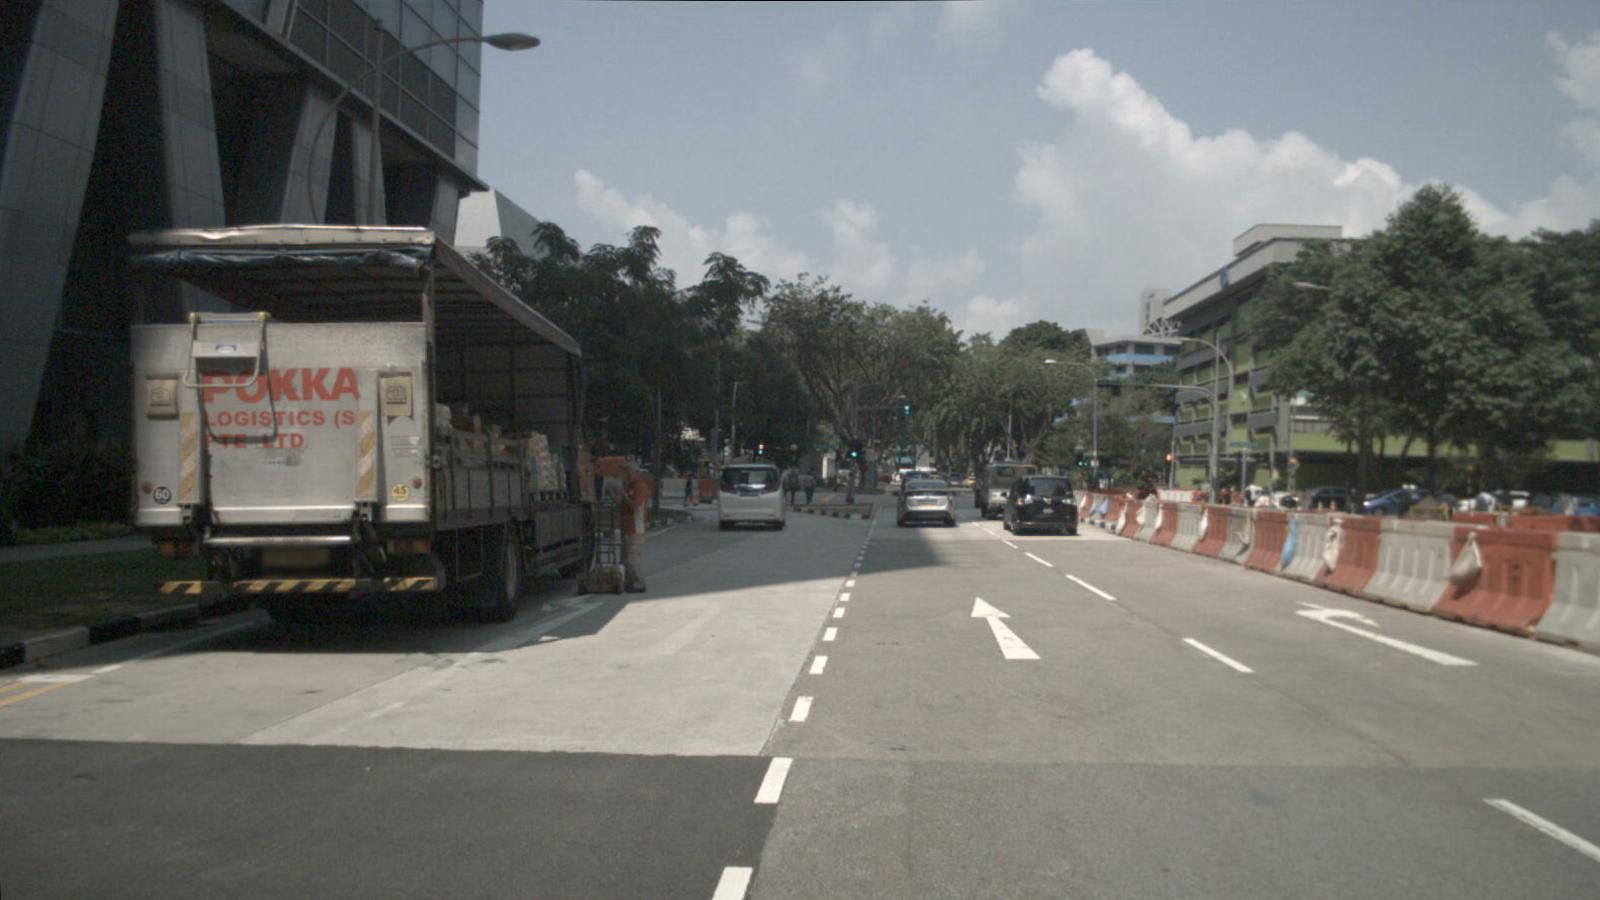
\includegraphics[width=\textwidth]{images/methodology/raw_image_0.jpg}
        \caption{}
        \label{fig:raw_pointcloud_a}
    \end{subfigure}
    \hfill
    \begin{subfigure}[b]{0.45\textwidth}
        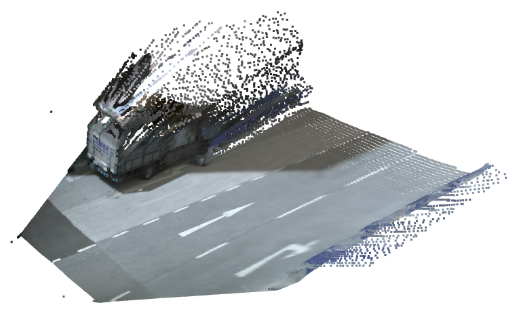
\includegraphics[width=\textwidth]{images/methodology/pcd_raw.png}
        \caption{}
        \label{fig:raw_pointcloud_b}
    \end{subfigure}

    \caption{Source image (a) and reconstructed pointcloud (b).}
    \label{fig:raw_pointcloud}
\end{figure}

\subsubsection{Instance scene PCD}

The objective of this module is to compute instance-level point clouds from the previously reconstructed scene point cloud using the corresponding semantic mask of the input perspective image (obtained as one of the BEV2Seg\_2 module's output). The semantic and geometric information is fed into this module, where instance differentiation is performed for specific object classes as shown in Figure~\ref{fig:instance_scene_diagram}. This enables the isolation of individual instance point clouds and the computation of their enclosing cuboids. The resulting panoptic point cloud provides a 3D object-level representation of the scene, which can be used as input for subsequent modules. It is also interesting to point out this is achieved from a single monocular image, demonstrating the system's capability for 3D object detection without requiring multi-view or stereo data.

\begin{figure}[h!]
    \centering
    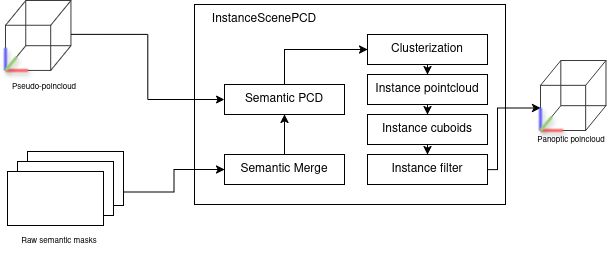
\includegraphics[width=0.6\linewidth]{images/methodology/instance_scene_flow_diagram.png}
    \caption{Instance scene computation diagram.}
    \label{fig:instance_scene_diagram}
\end{figure}

Firstly, the input semantic mask is preprocessed with a label merging step in which semantically similar labels are unified under a single target class. This step helps mitigate noise and inconsistencies in the model's predictions, which could negatively impact the subsequent instance estimation process. The merging policy is defined by default as shown in Table~\ref{tab:merge_dict}. For example, the target class \texttt{vehicle.car} gathers all NuScenes vehicle categories that seem like cars, such as buses, trucks, trailers, and emergency vehicles.

\begin{table}[h!]
    \centering
    \footnotesize
    \begin{tabular}{|l|p{10cm}|}
        \hline
        \textbf{Merged Class} & \textbf{Original Classes} \\
        \hline
        \texttt{background} & \texttt{background} \\ 
        \hline
        \texttt{animal} & \texttt{animal} \\
        \hline
        \texttt{human.pedestrian} &
        \texttt{human.pedestrian.adult}, \texttt{human.pedestrian.child}, \texttt{human.pedestrian.construction\_worker}, \texttt{human.pedestrian.personal\_mobility}, \texttt{human.pedestrian.police\_officer}, \texttt{human.pedestrian.stroller}, \texttt{human.pedestrian.wheelchair} \\
        \hline
        \texttt{movable\_object.barrier} &
        \texttt{movable\_object.barrier}, \texttt{movable\_object.debris}, \texttt{movable\_object.pushable\_pullable}, \texttt{movable\_object.trafficcone}, \texttt{static\_object.bicycle\_rack}, \\
        \hline
        \texttt{vehicle.car} & 
        \texttt{vehicle.bus.bendy}, \texttt{vehicle.bus.rigid}, \texttt{vehicle.car}, \texttt{vehicle.construction}, \texttt{vehicle.emergency.ambulance}, \texttt{vehicle.emergency.police}, \texttt{vehicle.trailer}, \texttt{vehicle.truck} \\
        \hline
        \texttt{vehicle.ego} & \texttt{vehicle.ego} \\
        \hline
        \texttt{vehicle.motorcycle} & 
        \texttt{vehicle.bicycle}, \texttt{vehicle.motorcycle} \\
        \hline
        \texttt{flat.driveable\_surface} & \texttt{flat.driveable\_surface} \\
        \hline
    \end{tabular}
    \caption{Class merge dictionary used for semantic simplification.}
    \label{tab:merge_dict}
\end{table}

Once the semantic mask has been preprocessed and the point cloud computed, a pre-filtering step is applied to remove points that fall outside predefined bounds (by default, $\left[10, 5, 30\right]$ meters in the $\hat{x}_c$, $\hat{y}_c$, and $\hat{z}_c$ axes). Then, the semantic mask is projected onto the point cloud to create a semantic point cloud. This process is straightforward, as each 3D point is associated with the corresponding semantic label based on the pixel indices. As a result, each 3D point is labeled with its appropriate semantic class (see Figure~\ref{fig:semantic_pointcloud_a}). Additionally, each semantic point cloud is tagged with a "dynamic" flag, which indicates whether the associated object is likely to move. Only 3D semantic points with this flag set are passed through the instance detection process. This helps avoid unnecessary processing of labels such as background, road barriers, or driveable areas.

\begin{figure}[h!]
    \centering
    \begin{subfigure}[b]{0.45\textwidth}
        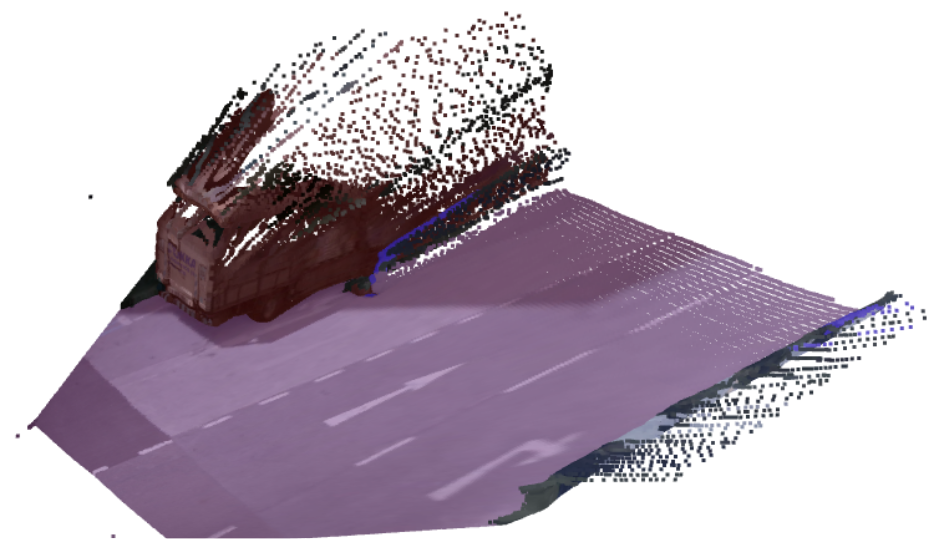
\includegraphics[width=\linewidth]{images/methodology/pcd_semantic.png}
        \caption{}
        \label{fig:semantic_pointcloud_a}
    \end{subfigure}
    \hfill
    \begin{subfigure}[b]{0.45\textwidth}
        
\includegraphics[width=\textwidth]{images/shared/no_signal.jpg}
        \caption{}
        \label{fig:semantic_pointcloud_b}
    \end{subfigure}

    \caption{Colorized semantic pointcloud (a) and denoised pointcloud with instance detection (b).}
    \label{fig:semantic_pointcloud}
\end{figure}

The instance detection process (Algorithm~\ref{algorithm:instance_pointcloud}) faces two key challenges: extracting individual instances from dynamic semantic point clouds and mitigating the inherent noise and artifacts that result from the depth estimation process. To address this, the DBSCAN clustering algorithm is employed. It effectively extracts distinct instances from each dynamic semantic point cloud, removes noisy outlier points and minimizes the "trail" artifacts commonly left by depth estimation along object edges, as illustrated in Figure~\ref{fig:semantic_pointcloud_b}. Then, for each computed instance point cloud, the minimal camera \aclink{AABB} is calculated by taking the minimum and maximum coordinates along each of the camera axes $\hat{x}_c$, $\hat{y}_c$, and $\hat{z}_c$. Oriented bounding boxes were not used in this work.

Estimating the correct orientation of a bounding box is a challenging task, especially when only a partial view of the object is available (see Figure~\ref{fig:oriented_bounding_box_problems}). Depending on the viewpoint and the amount of visible surface, traditional methods are very likely to produce inaccurate orientation estimates. Modern 3D object detection models typically address this issue by learning the statistical distribution of common object shapes and orientations. Datasets like NuScenes even provide metrics such as Average Scale Error and Average Orientation Error to evaluate the accuracy of these predictions.

However, the main goal in this thesis is to estimate the physical space occupied by a vehicle in the scene for pre-annotation purposes, not precise orientation or object alignment. In this context, using an \aclink{AABB} may slightly overestimate the occupied space when objects are not aligned with the camera's reference frame, for example during turns or when vehicles are parked at an angle. Nevertheless, this estimation does not pose a significant problem since these overestimated regions are not of special interest in the annotation process.

\begin{figure}[h!]
    \centering
    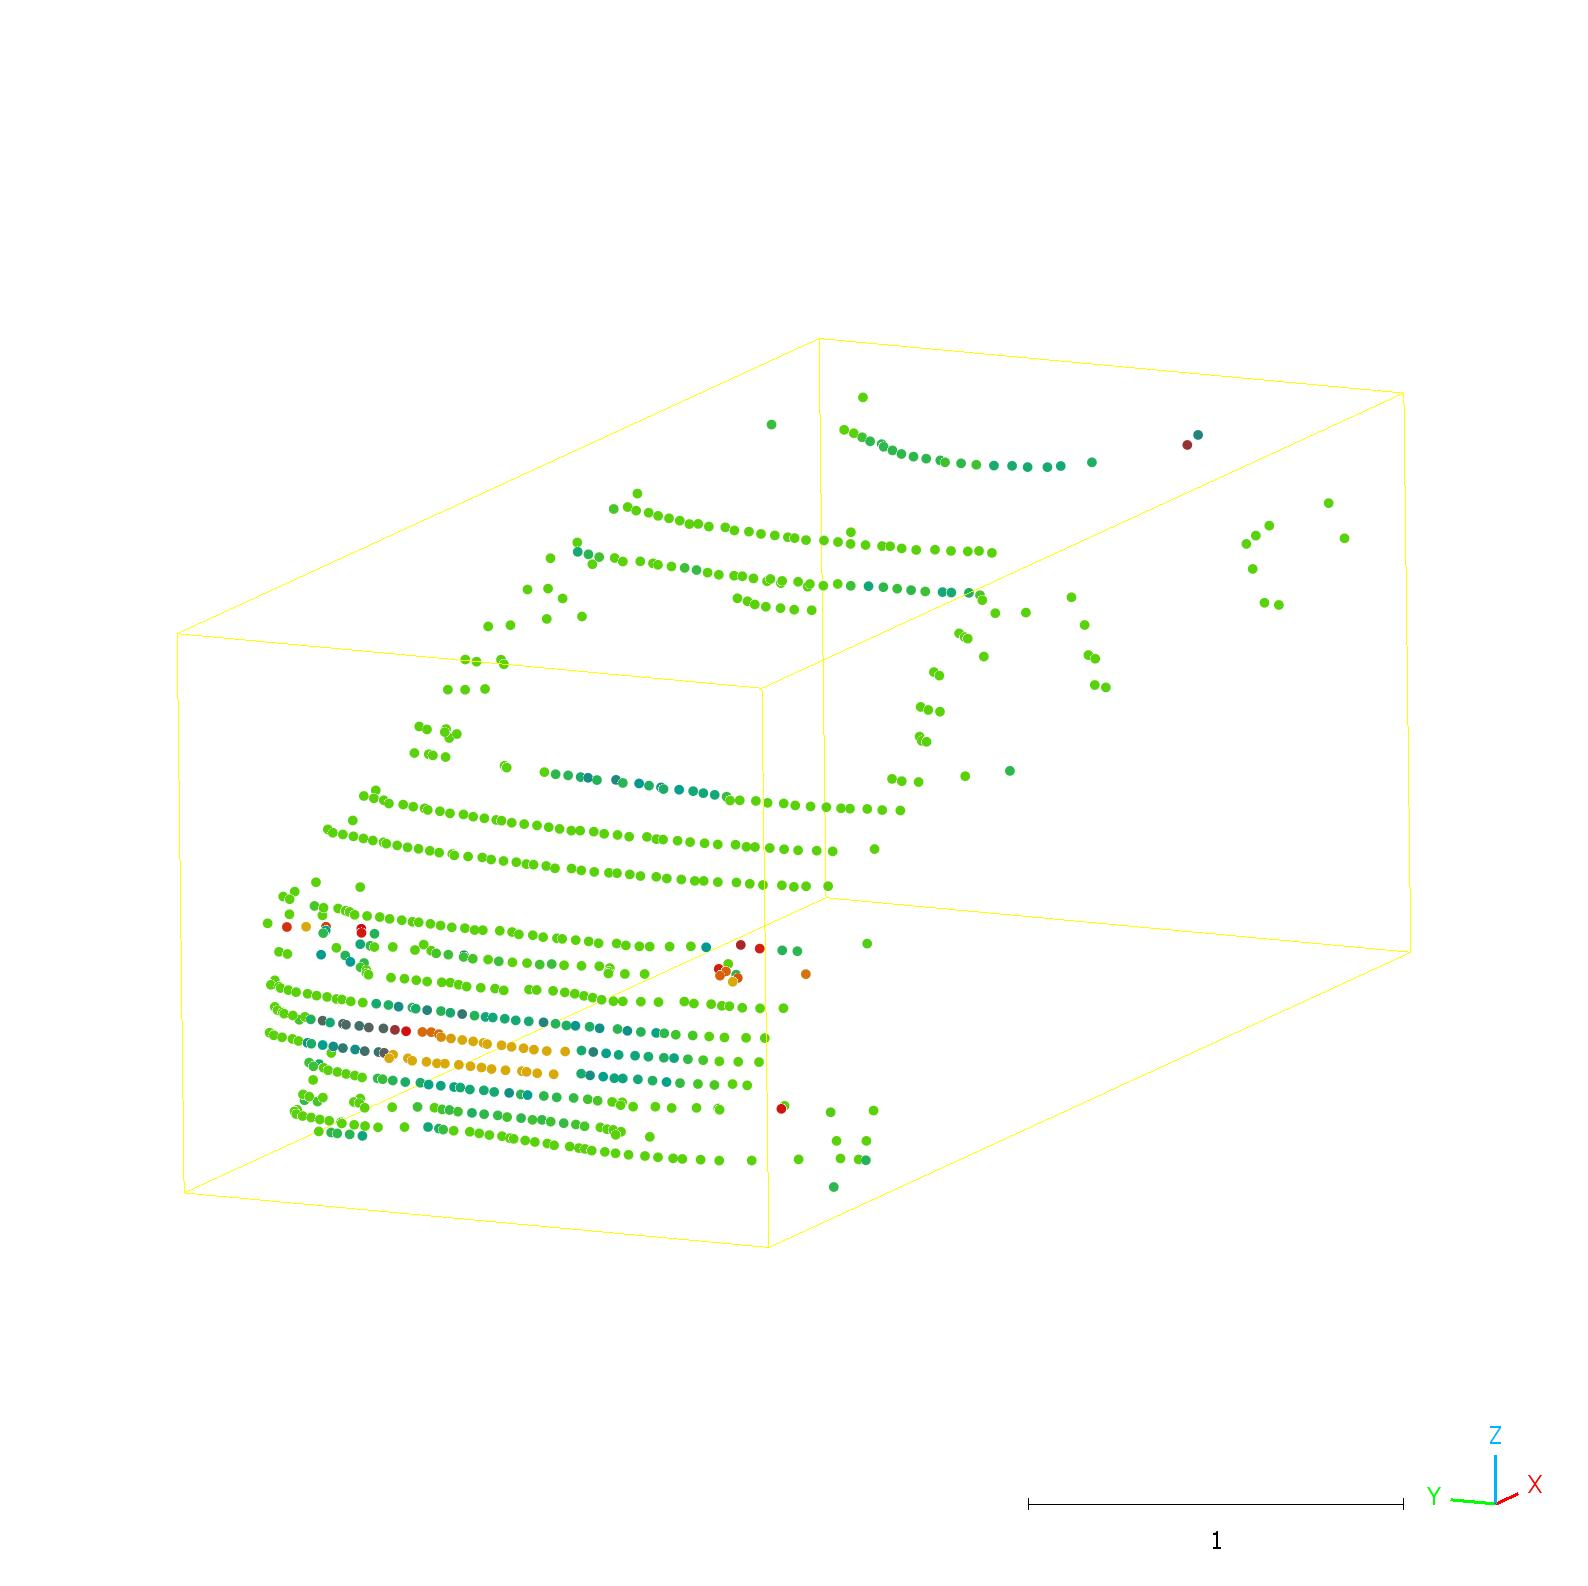
\includegraphics[width=0.5\linewidth]{images/methodology/oriendet_bbox_problem_aux.jpeg}
    \caption{Oriented bounding box problems.}
    \label{fig:oriented_bounding_box_problems}
\end{figure}

\hl{Change oriented bounding box problems figure. Complete this algorithm.}
\begin{algorithm}
    \caption{Instance Pointcloud Computation}
    \label{algorithm:instance_pointcloud}
    \footnotesize

    \begin{algorithmic}[1]
        \State \textbf{Input:} $P^{inst}$ panoptic pointcloud
        \State \textbf{Output:} $P^{inst}$ filtered panoptic pointcloud
        
        \For{$label \text{ in } P^{inst}$}
            \For{$i \text{ in } P^{inst}\left[label\right]$}
                \State $B \gets $
            
            \EndFor
        \EndFor
        
        \State \Return $P$
    \end{algorithmic}
\end{algorithm}

Finally, a filtering process is performed to ensure there are no noisy, redundant, too far away or floating instances. Also, it ensures there are no overlapping bounding boxes by checking each new instance's 3D bounding box against those already accepted. If an overlap is detected, the function compares their sizes: the larger box is kept, and the smaller one is removed or ignored. This helps avoid redundant or conflicting instances that may represent the same object or spatial region, improving the clarity and consistency of the data. The final results of this module are shown in Figure~\ref{fig:instance_scene_images}.

\begin{figure}[h!]
    \centering
    \begin{subfigure}[b]{0.45\textwidth}
        
\includegraphics[width=\textwidth]{images/shared/no_signal.jpg}
        \caption{}
        \label{fig:instance_scene_images_a}
    \end{subfigure}
    \hfill
    \begin{subfigure}[b]{0.45\textwidth}
        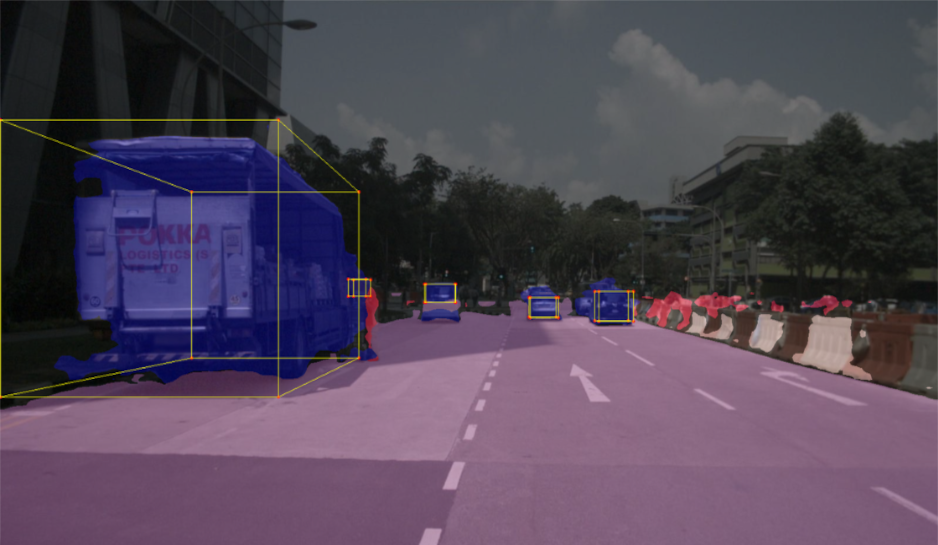
\includegraphics[width=\textwidth]{images/methodology/raw_cuboid_1.png}
        \caption{}
        \label{fig:instance_scene_images_b}
    \end{subfigure}

    \caption{Resulting instances in 3D (a) and projected into the front camera (b).}
    \label{fig:instance_scene_images}
\end{figure}


\subsubsection{Instance BEV mask}
Once the 3D instance detection is performed and the panoptic point cloud is generated, the final occupancy and occlusion masks can be estimated using the semantic \aclink{BEV} masks.

To associate the \aclink{BEV} semantic masks with the detected 3D instances, the semantic masks are first processed using a connected components labeling algorithm, which extracts the individual, non-connected regions for each semantic class. Then, for each instance in the panoptic point cloud, the base of its 3D bounding box is obtained and an intersection factor is calculated between each pair of base bounding boxes and connected mask regions. Using this intersection measure, the base polygons and connected masks are associated accordingly so each mask is related to one polygon but a polygon may have multiple masks. This is represented in Algorithm~\ref{algorithm:occ_masks} and results in a final representation of occupancy, defined by the base of the 3D bounding box, and occlusion, which is captured by the distorded shape of the semantic mask from the \aclink{BEV} perspective.

A single cuboid base can be associated with multiple \aclink{BEV} masks because a 3D instance may appear fragmented in the \aclink{BEV} semantic view. When connected components labeling is applied to these masks, each fragment is identified as a separate region. However, since all fragments originate from the same 3D object, they are associated with the same cuboid base.

\hl{Complete this algorithm.}
\begin{algorithm}
    \caption{Occupancy Occlusion masks}
    \label{algorithm:occ_masks}
    \footnotesize

    \begin{algorithmic}[1]
        \State \textbf{Input:} 
        \State \textbf{Output:} 
        \State \Return $x$
    \end{algorithmic}
\end{algorithm}

This method allows for estimating the vehicle’s extent while handling certain ambiguities. For example, when a vehicle is perfectly aligned with the camera view, only the rear width and height are clearly visible (see Figure~\ref{fig:oriented_bounding_box_problems}), making the depth extent estimation ambiguous. However, when the vehicle is rotated relative to the camera, its dimensions become more discernible. In such cases, the 3D detection phase, despite the ovestimation of \aclink{AABB}, enables a more reliable approximation of the vehicle's actual footprint.

\begin{figure}[h!]
    \centering
    \begin{subfigure}[b]{0.22\textwidth}
        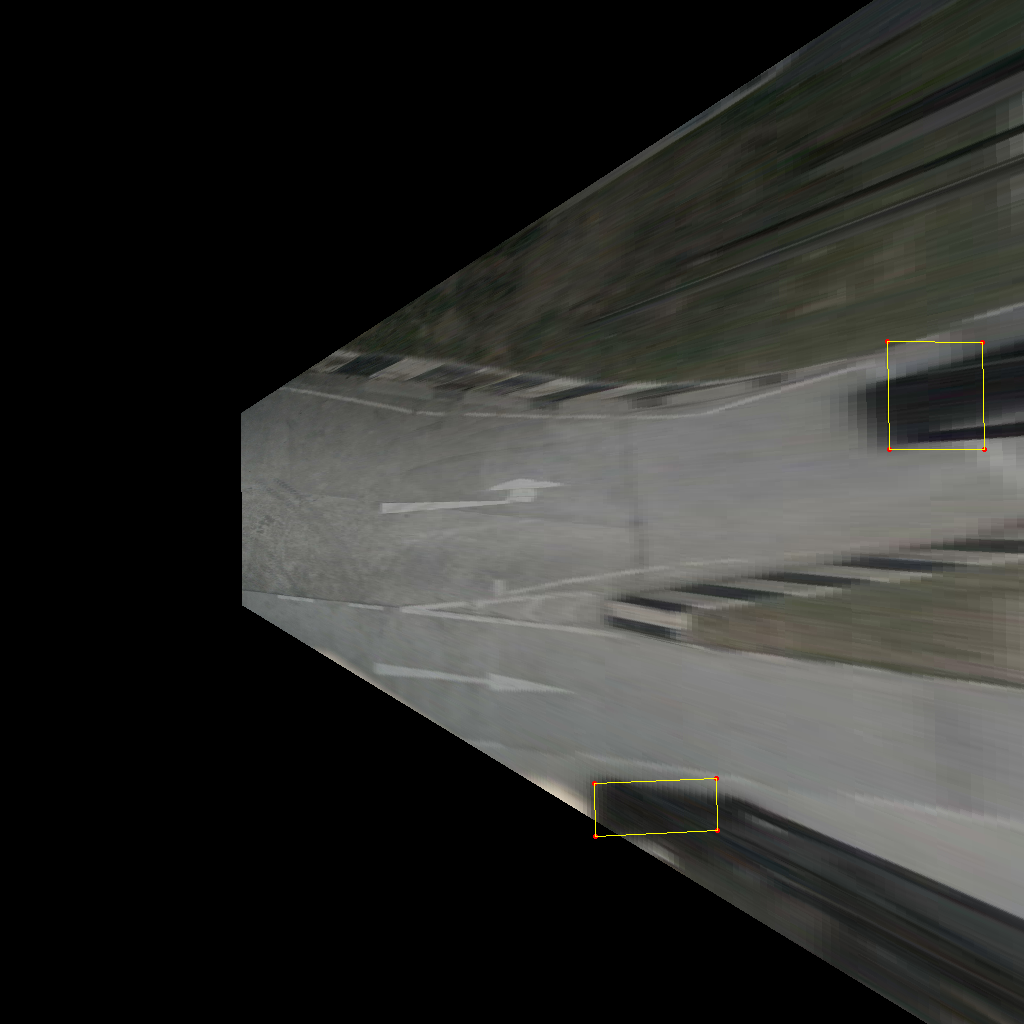
\includegraphics[width=\textwidth]{images/methodology/bev_occupancy_oclusion/bev_cuboid_9.png}
        \caption{}
        \label{fig:bev_occupancy_occlusion_a}
    \end{subfigure}
    \hfill
    \begin{subfigure}[b]{0.22\textwidth}
        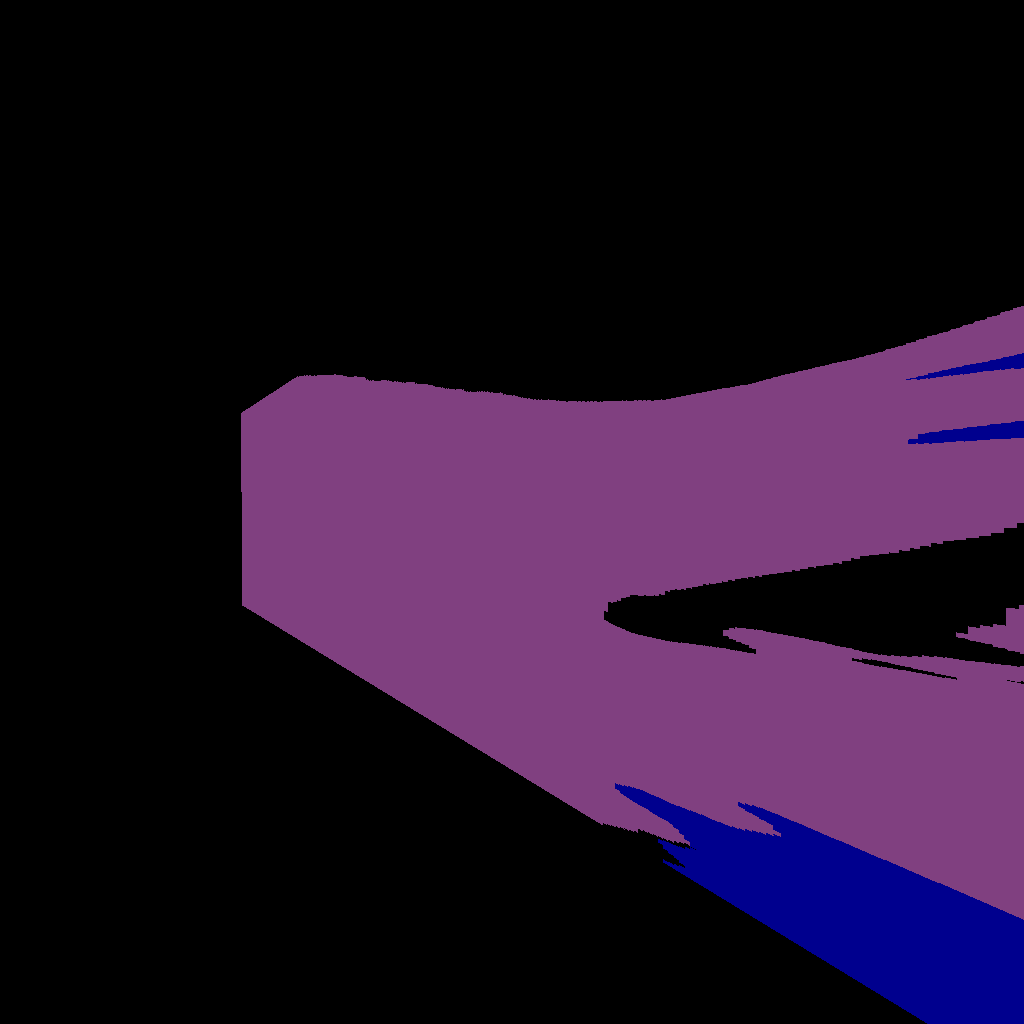
\includegraphics[width=\textwidth]{images/methodology/bev_occupancy_oclusion/bev_semantic_color_9.png}
        \caption{}
        \label{fig:bev_occupancy_occlusion_b}
    \end{subfigure}
    \hfill
    \begin{subfigure}[b]{0.22\textwidth}
        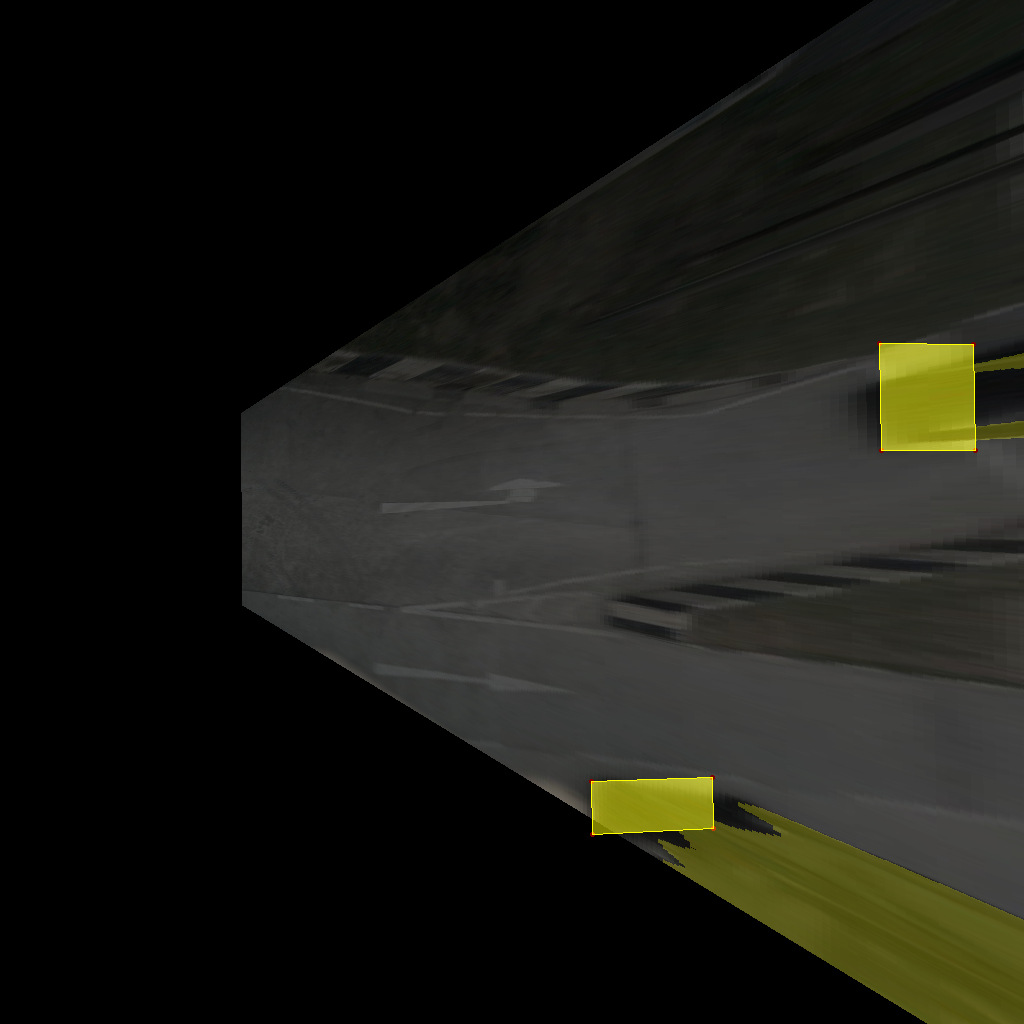
\includegraphics[width=\textwidth]{images/methodology/bev_occupancy_oclusion/bev_occ_9.png}
        \caption{}
        \label{fig:bev_occupancy_occlusion_c}
    \end{subfigure}
    \hfill
    \begin{subfigure}[b]{0.22\textwidth}
        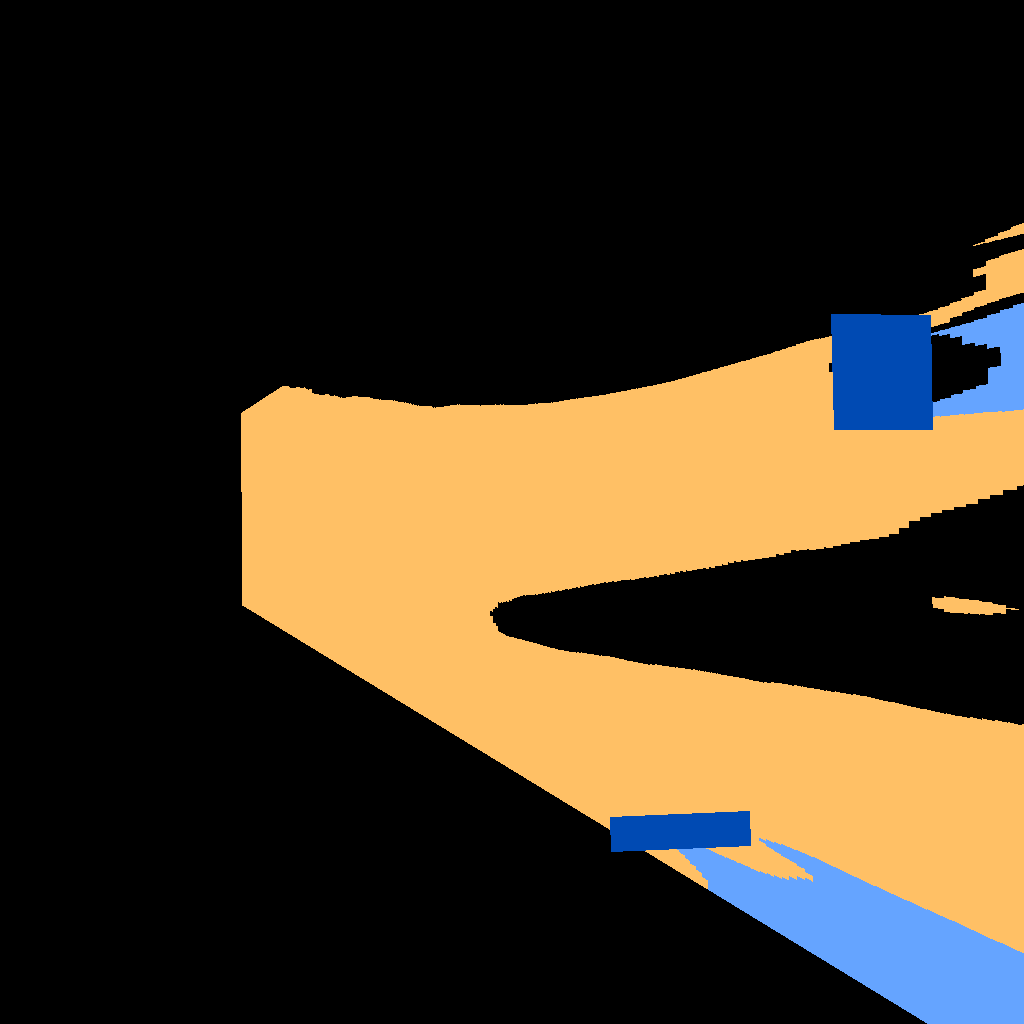
\includegraphics[width=\textwidth]{images/methodology/bev_occupancy_oclusion/dt_occ_mask_colored_9.png}
        \caption{}
        \label{fig:bev_occupancy_occlusion_d}
    \end{subfigure}

    \caption{BEV occupancy and occlusion masks. (a) Input 3D detections; (b) input BEV semantic masks; (c) BEV occupied-occluded connected components and (d) final rasterized BEV mask.}
    \label{fig:bev_occupancy_occlusion}
\end{figure}


Finally, these estimated occupancy and occlusion masks are rasterized onto the \aclink{BEV} drivable area mask, which is obtained from the initial semantic segmentation step. This final overlay adheres to the specific labeling scheme detailed in Table~\ref{tab:occ2_labels}. The entire process, from initial detections to the final composite BEV mask, is visually summarized in Figure~\ref{fig:bev_occupancy_occlusion}.

\begin{table}[h]
    \centering
    \begin{tabular}{l c c c c}
        \toprule
        \textbf{Name} & \textbf{ID} & \textbf{Color (RGB)} \\
        \midrule
        background  & 0 & (0, 0, 0)         \\
        occuped     & 1 & (0, 74, 179)      \\
        occluded    & 2 & (101, 164, 255)   \\
        driveable   & 3 & (255, 192, 101)   \\

        \bottomrule
    \end{tabular}
    \caption{Semantic labels defined for resulting masks}
    \label{tab:occ2_labels}
\end{table}

\subsubsection{Evaluation strategy}
As early mentioned, the final objective of the annotation pipeline is to provide occupancy, occlusion and driveable area masks. To achieve this, the process starts from semantic masks of the environment, both in the camera and \aclink{BEV} domains. A crucial intermediate step in this pipeline is the 3D object detection from monocular images in the camera view to estimate the dimensions and positions of obstacles. As this detection is performed using pointcloud clustering algorithms it is particularly important to assess its performance using appropriate evaluation metrics.

Another key aspect of the evaluation involves assessing the quality of the generated \aclink{BEV} masks. Therefore, the evaluation methodology must address two distinct components: the accuracy of the monocular 3D object detection, and the fidelity of the resulting \aclink{BEV} masks when compared to a defined ground truth. This evaluation uses the pipeline's output OpenLabel file for a vehicular scene, alongside the corresponding ground truth OpenLabel file which contains annotated elements. A 'vehicular scene' is defined here as a sequence of frames with annotations that include not only the environment, but also vehicle position and odometry.

\subsubsubsection{3D detections evaluation} \label{sec:3d_det_evaluation}

The NuScenes metrics~\cite{nuscenes} were considered as a starting point as this dataset was specifically developed to facilitate the training and evaluation of 3D perception strategies. A central component of its evaluation policy is the matching between predictions and ground truth, which is performed using the 2D distance between the centers of the predicted and ground truth bounding boxes projected onto the ground plane. A prediction is considered a true positive if this distance falls below a predefined threshold. Then, \aclink{AP} is computed across several distance thresholds ($\{0.5, 1, 2, 4\}$ meters), and the final \aclink{mAP} score is obtained by averaging \aclink{AP} values over all object classes.

Beyond the \aclink{mAP}, NuScenes includes additional metrics to evaluate key attributes of correctly detected objects, using a fixed association threshold of $2$ meters. These include translation, scale, orientation, velocity, and attribute classification errors. Each of these metrics targets a specific aspect of detection performance, such as localization accuracy or motion estimation. To provide a unified performance score, the NuScenes Detection Score aggregates all these metrics into a single weighted average, offering a comprehensive view of system performance.

Nevertheless, the use case addressed in this work diverges significantly from the standard NuScenes benchmark. Since 3D detections are performed from monocular images via clustering, the resulting cuboids inherently represent only the visible portion of objects from the camera's perspective. This makes centroid-based 3D box evaluation less meaningful due to an expected displacement between prediction and ground truth. Additionally, the camera-aligned nature of these cuboids makes the orientation error metric impractical. Consequently, the evaluation strategy of this 3D detections is focused on the precision of the estimated cuboid dimensions and positions, which directly assesses the pipeline's ability to achieve reasonable detection accuracy.

In this scenario, employing centroid distance as the criterion for evaluating position predictions with ground truth poses a significant challenge. Therefore, a more suitable metric, the volume-to-volume distance (v2v), has been adopted. This metric is defined as the minimum distance between the convex hulls of the considered volumes (Figure~\ref{fig:bbox_disparity_b}).

However, the v2v metric has a notable limitation: it yields a value of zero whenever there is any intersection between the volumes, regardless of the degree of overlap. To overcome this, we utilize the Bounding Box Disparity (BBD) metric \cite{bounding_box_disparity}, which combines IoU and v2v into a single, continuous, and non-negative measure. This metric allows for the quantification of dissimilarity between two cuboids, whether they overlap or not. As stated in its original definition, while IoU can only compare intersecting cuboids, BBD provides a disparity measure even in the absence of overlap. Its interpretation is as follows:

\begin{equation}
    \begin{aligned}
    \text{BBD} = 1 - \text{IoU} + v2v
    \end{aligned}
    \label{eq:3d_metrics}
\end{equation}

\begin{itemize}
    \item If $BBD = 0$, the cuboids are identical (total intersection).
    \item If $0 < BBD < 1$, there is overlap but also disparity.
    \item If $BBD \geq 1$, the cuboids do not overlap.
\end{itemize}

These distinct cases are illustrated in Figure~\ref{fig:bbox_disparity}.

\begin{figure}[h!]
    \centering
    \begin{subfigure}[b]{0.45\textwidth}
        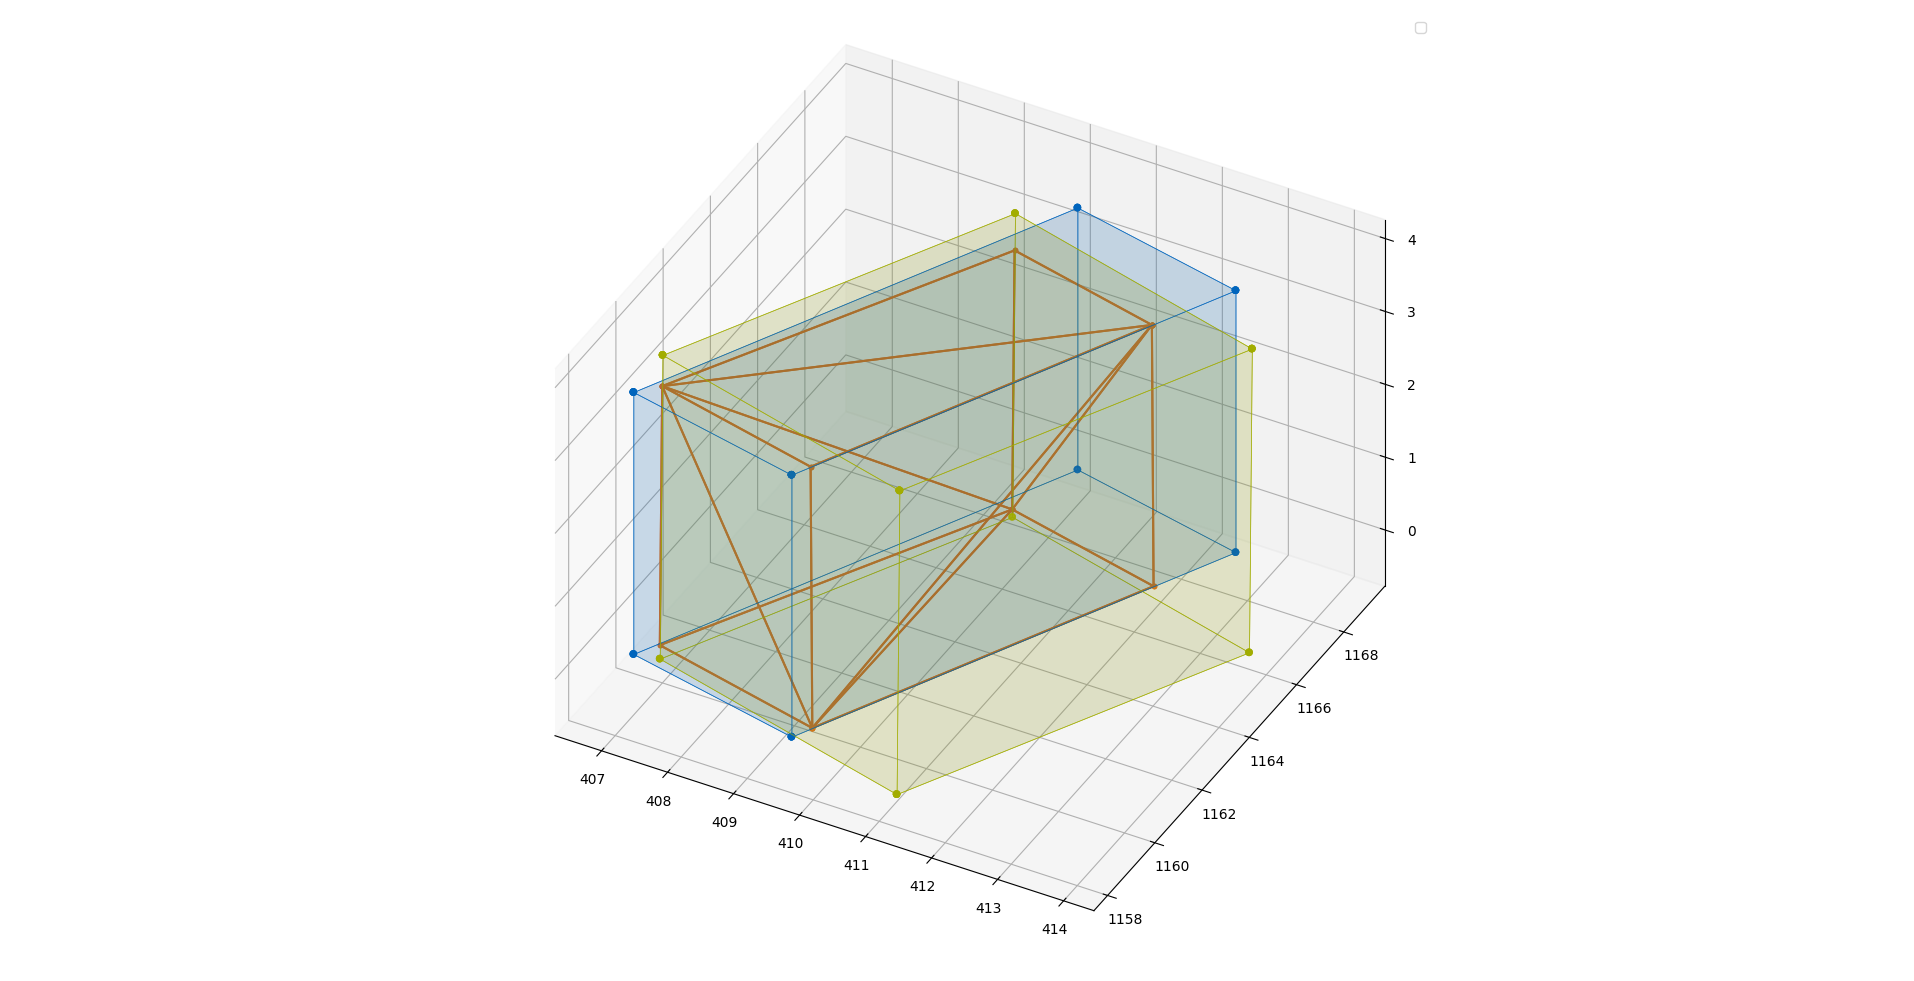
\includegraphics[width=\textwidth]{images/methodology/frame_0_3d_bb.png}
        \caption{}
        \label{fig:bbox_disparity_a}
    \end{subfigure}
    \begin{subfigure}[b]{0.45\textwidth}
        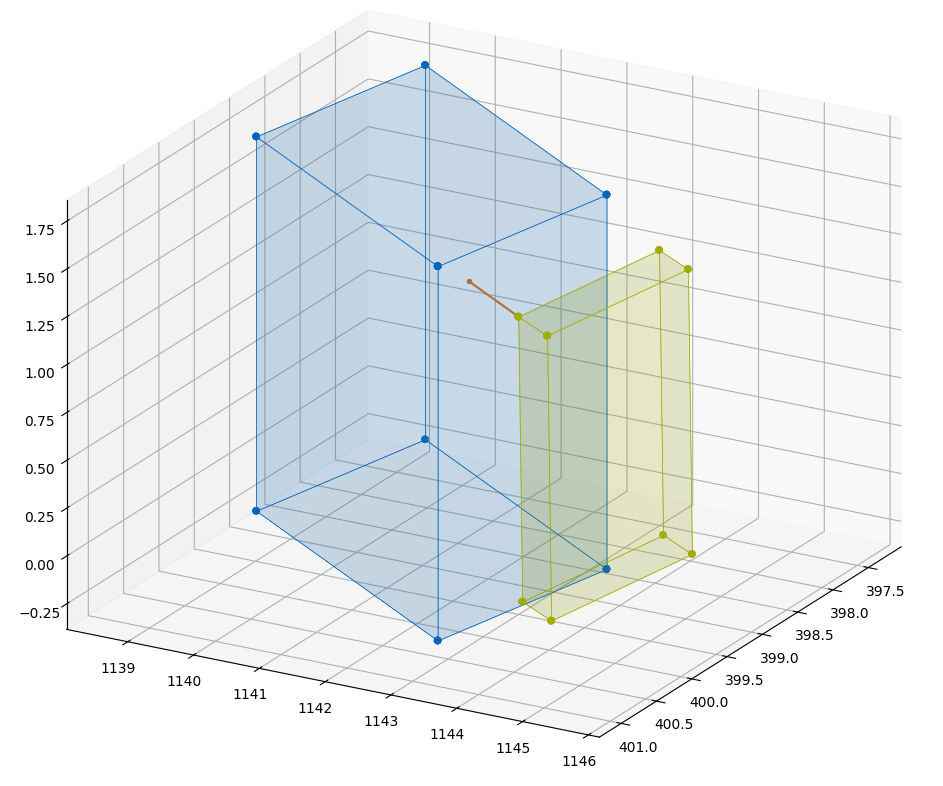
\includegraphics[width=\textwidth]{images/methodology/frame_2_3d_bb.png}
        \caption{}
        \label{fig:bbox_disparity_b}
    \end{subfigure}
    \caption{Bounding Box Disparity scene calculation. (a) shows an example of intersection, while (b) shows an example of volumetric distance}
    \label{fig:bbox_disparity}
\end{figure}

On the other hand, to evaluate the error in the estimation of the detected object's dimensions, the absolute difference between the dimensions of the predicted and ground truth cuboids along each axis (length, width, and height) has been considered. This allows for the analysis of which dimension exhibits the greatest error and under what conditions.

The evaluation process begins by defining the spatial region in which the detections produced by the pipeline will be considered. Since the system is capable of generating predictions at distances greater than those actually used for producing the \aclink{BEV} occupancy and occlusion masks, the evaluation range is restricted to the same area used for generating those masks. Specifically, this involves projecting the camera's field of view onto the ground plane and limiting the maximum detection distance to 15 meters. As a result, only the predictions and ground truth elements that fall within this projected polygon at a given time frame are included in the evaluation.

Then, the matching between predictions and ground truth is performed, formalized as a Linear Sum Assignment Problem (LSAP) and solved using the Hungarian algorithm. Because of this, the cost matrix is initially calculated as the v2v distance between all ground truth and prediction instances.  However, unlike a standard LSAP, this implementation incorporates a maximum distance threshold for valid assignments. Detections with no sufficiently close ground truth counterparts are removed before solving the LSAP, and the cost matrix is padded to a square shape. Finally, assignments exceeding the distance threshold are discarded after the LSAP solution, ensuring only meaningful matches are retained. 
\hl{Maybe it is interesting to add an Appendix about this}

Finally, the following metrics are calculated:
\begin{itemize}
    \item \textbf{TP/FP/FN}: Computed from prediction-ground truth associations.
    \item \textbf{DD}: Volume difference between associated cuboids.
    \item \textbf{DED}: Absolute difference per axis (length, width, height).
    \item \textbf{v2v}: Minimum distance between convex hulls.
    \item \textbf{IoU}: 3D intersection-over-union.
    \item \textbf{BBD}: Dissimilarity metric for overlapping/non-overlapping boxes.
\end{itemize}


\subsubsubsection{BEV masks evaluation}
To evaluate the occupancy, occlusion, and drivable area masks, it is necessary to generate corresponding ground truth masks. These masks are computed from the OpenLABEL annotated vehicular scene data as follows. For each frame, only the elements visible to the camera are considered (as detailed in Section~\ref{sec:3d_det_evaluation}) and a custom algorithm is applied to process this visible information.

This algorithm calculates camera viewing angles along the $\hat{x}_c$ axis to define $N$ rays. A step length $h$ is also defined, which determines the intervals at which each ray will sample points to classify them as visible, occluded, or belonging to an occupied area. All rays originate from the camera coordinate frame and are subsequently transformed to the vehicle's coordinate frame as it is the coordinate system in which the \aclink{BEV} masks are generated (see Section\ref{sec:BEVDataset}).

Once these rays and their corresponding check points are established in the \aclink{BEV} mask coordinate frame, the point classification process begins. An iteration process goes through camera-visible objects (also transformed to the vehicle coordinate frame) and check if the base of the object's bounding box contains each ray's point. Here, three outcomes are possible: no intersection, indicating a visible point; intersection, classifying the point as occupied; or no current intersection but a previous intersection along the same ray, resulting in occlusion classification.


Following ray point evaluation, closed polygon sets are constructed to represent all points within each of the three classes. A clustering algorithm groups points of the same class to distinguish connected areas and generate individual sub-polygons. These sub-polygons are formed using only the edge points of each cluster and finally, the ground truth drivable area, which is directly annotated as polygons, undergoes a simpler process of identifying camera-visible polygons. All polygon sets are then rasterized into semantic masks, adhering to the used \aclink{BEV} parameters and considering the semantic classes described in Table~\ref{tab:occ2_labels}. This whole process is represented in Figure~\ref{fig:gt_occ2_masks}.  

\begin{figure}[htbp]
    \centering
    \begin{subfigure}[b]{0.3\textwidth}
        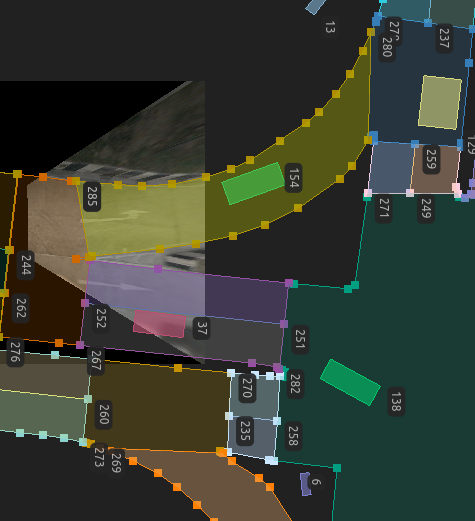
\includegraphics[width=\textwidth, height=\textwidth]{images/methodology/gt_occ2_maks/WebLABEL_bev_8.png} 
        \caption{}
        \label{fig:gt_occ2_masks_a}
    \end{subfigure}
    \hfill
    \begin{subfigure}[b]{0.3\textwidth}
        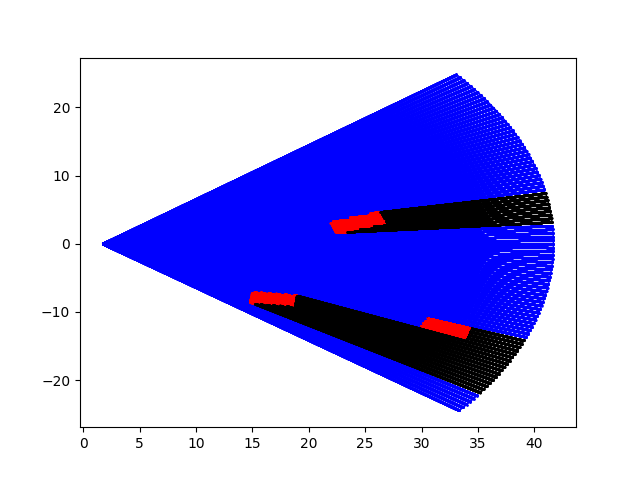
\includegraphics[width=\textwidth, height=\textwidth]{images/methodology/gt_occ2_maks/gt_vec_mask_8.png}
        \caption{}
        \label{fig:gt_occ2_masks_b}
    \end{subfigure}
    \hfill
    \begin{subfigure}[b]{0.3\textwidth}
        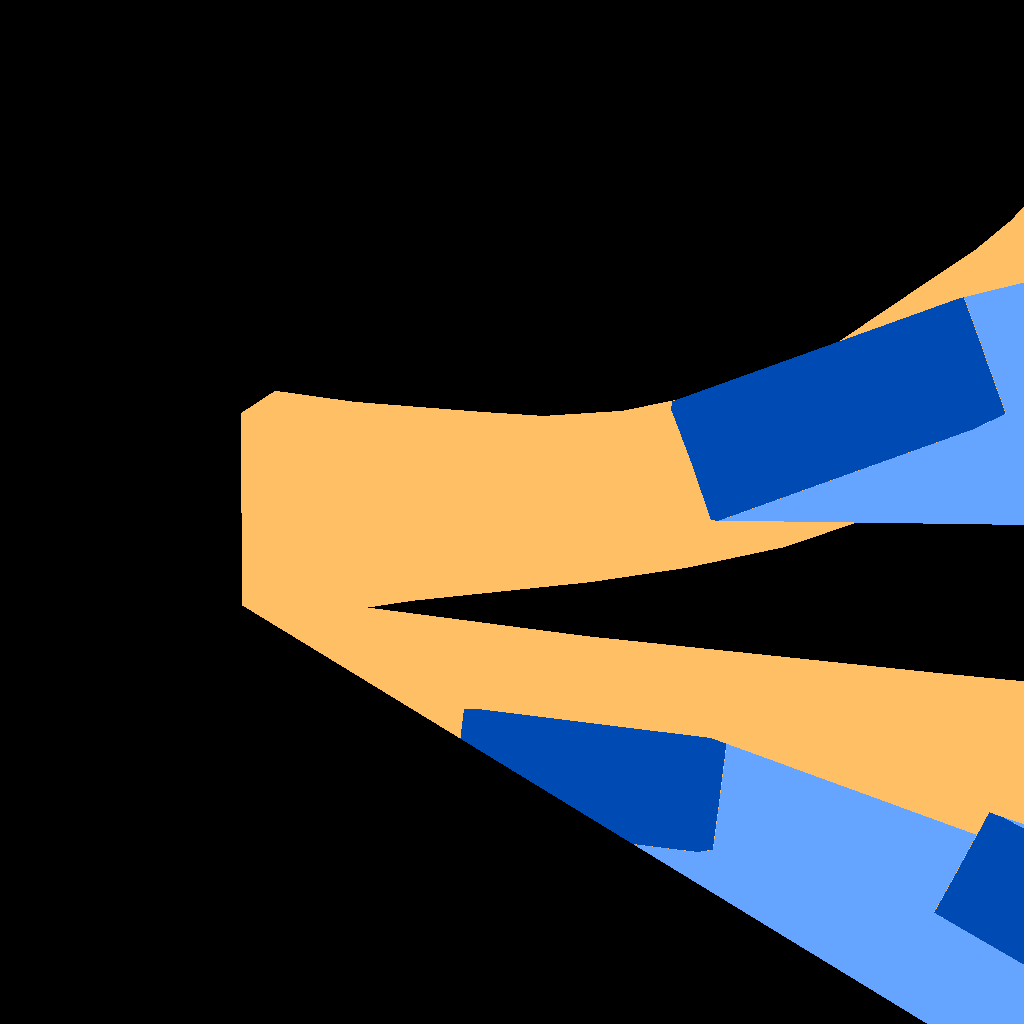
\includegraphics[width=\textwidth, height=\textwidth]{images/methodology/gt_occ2_maks/gt_occ_mask_colored_8.png}
        \caption{}
        \label{fig:gt_occ2_masks_c}
    \end{subfigure}

    \caption{BEV ground truth masks: (a) WebLABEL visualization, (b) resulting polygons, (c) rasterized and colored BEV mask.}
    \label{fig:gt_occ2_masks}
\end{figure}
